\chapter{Calcul intégral}
\chaptertoc

\section{Intégrale sur un segment}

    \begin{defi}{Subdivision}{}
        Une \textbf{subdivision} du segment $\intervalleFF{a}{b}$ est une suite finie 
        \[ \sigma =  (x_0, x_1,\ldots,x_n) \] telle que $x_0 = a$, $x_n = b$ et $x_0 < x_1 < \ldots < x_n$.
    \end{defi}

    \begin{defi}{Fonction en escalier}{}
        Une fonction $f \in \mathcal{F}(\intervalleFF{a}{b}, \mathbb{R})$ est dite \textbf{fonction en escalier} si 
        \[ \exists \, \sigma(\intervalleFF{a}{b}), \, \forall i \in \intervalleEntier{1}{n}, \, f \vert_{\intervalleOO{x_{i-1}}{x_i}} \text{ est constante} \]
        La subdivision $\sigma$ est dite adaptée à $f$. 
        
        On notera ici $\mathcal{E}(\intervalleFF{a}{b},\mathbb{R})$ l’ensemble des fonctions en escalier de $\intervalleFF{a}{b}$.
    \end{defi}

    \begin{omed}{Notation}{myyellow}
        \begin{soient} 
            \item $\intervalleFF{a}{b}$ un segment de $\mathbb{R}$,
            \item $f$ une fonction en escalier sur $\intervalleFF{a}{b}$,
            \item $\sigma = (x_0,x_1,\ldots,x_n)$ une subdivision adaptée à $f$,
            \item $\forall i \in \intervalleEntier{1}{n}, \, \alpha_i$ la valeur de $f$ sur $\intervalleOO{x_{i-1}}{x_i}$.
        \end{soient}
        On note 
        \[  I(\sigma,f) = \sum\limits_{i=1}^n \alpha_i (x_i - x_{i-1}) \]
    \end{omed}

    \begin{defi}{Fonction continue par morceaux}{}
        Soient $\intervalleFF{a}{b}$ un segment de $\mathbb{R}$ et $f \in \mathcal{F}(\intervalleFF{a}{b},\mathbb{R})$.

        On dit que $f$ est \textbf{continue par morceaux} sur $\intervalleFF{a}{b}$ si 
        \[ \exists \,\sigma(\intervalleFF{a}{b}), \, \forall i \in \intervalleEntier{1}{n}, \left\{ \begin{array}{l} 
            f \vert_{\intervalleOO{x_{i-1}}{x_i}} \text{ est continue} \\
            f \text{ admet une limite finie}  \\
            \quad \text{à droite en } x_{i-1} \\
            \qquad \text{et à gauche en } x_i
        \end{array} \right. \]
        La subdivison est alors dite \textbf{adaptée} à $f$.

        On note $\CM(\intervalleFF{a}{b},\mathbb{R})$ l’ensemble des fonctions continues par morceaux sur $\intervalleFF{a}{b}$ à valeurs dans $\mathbb{R}$.
    \end{defi}

    \begin{prop}{}{}
        Toute fonction $f \in \CM(\intervalleFF{a}{b})$ est bornée.
    \end{prop}

    \begin{demo}{Preuve}{myolive}
        On considère $\sigma = (x_0, \ldots, x_n)$ une subdivision de $\intervalleFF{a}{b}$ telle que 
        \begin{itemize}
            \item $\forall i \in \intervalleEntier{0}{n-1}$, $\restr{f}{\intervalleOO{x_i}{x_{i-1}}}$ est continue.
            \item $ \forall i \in \intervalleEntier{0}{n}$, $\lim_{x \to x_i^-} f(x)$ et $\lim_{x \to x_i^+} f(x)$ existent.
        \end{itemize}
        Soit $i \in \intervalleEntier{0}{n-1}$. On peut prolonger continuement $f$ sur $\intervalleFF{x_i}{x_{i+1}}$. On note $g_i$ ce prolongement. Donc $g_i$ est bornée car continue sur un segment, et on peut poser 
        \[ m_i = \sup_{\intervalleFF{x_i}{x_{i+1}}} \abs{g_i} \]   
        Alors $\forall x \in \intervalleFF{a}{b}$, 
        \[ \abs{f(x)} \leq \max \left(\big\{ m_i , i \in \intervalleEntier{0}{n-1} \big\} \cup \big\{ \abs{f(x_i)} , i \in \intervalleEntier{0}{n-1} \big\} \right) \]
        Donc $f$ est bornée.
    \end{demo}

    \begin{theo}{Définition de l’intégrale}{}
        Soient $\intervalleFF{a}{b}$ un segment de $\mathbb{R}$ et $f \in \mathcal{C}_{pm}(\intervalleFF{a}{b},\mathbb{R})$.
        On note 
        \begin{align*}
            \mathcal{E}^-(f) &= \left\{ \int_{a}^{b} \varphi, \, \varphi \in \mathcal{E}(\intervalleFF{a}{b},\mathbb{R}),\, \forall t \in \intervalleFF{a}{b}, \, \varphi(t) \leq f(t) \right\} \\
         \mathcal{E}^+(f) &= \left\{ \int_{a}^{b} \psi, \, \psi \in \mathcal{E}(\intervalleFF{a}{b},\mathbb{R}), \, \forall t \in \intervalleFF{a}{b}, \, \psi(t) \geq f(t) \right\}
        \end{align*}
        \begin{alors}
            \item $\mathcal{E}^-(f)$ admet une borne supérieure $A(f)$.
            \item $\mathcal{E}^+(f)$ admet une borne inférieure $B(f)$.
            \item $A(f) = B(f)$.
        \end{alors}
        On appelle \textbf{intégrale} de $f$ sur $\intervalleFF{a}{b}$ la valeur commune de $A(f)$ et $B(f)$.

        On la note $\int_{a}^b f(t)dt$ ou $\int_a^b f$.

        Enfin on appelle valeur moyenne de la fonction sur $\intervalleFF{a}{b}$ le nombre $\frac{1}{b-a} \int_a^b f$.
    \end{theo}

\section{Propriétés de l’intégrale}

    \subsection{Propriétés fondamentales}

    \begin{prop}{Propriétés fondamentales de l’intégrale}{}
        Soient $(a,b) \in \mathbb{R}^2$ et $f,g \in \CM(\intervalleFF{a}{b},\mathbb{R})$. 

        \begin{enumerate}
            \item Linéarité de l’intégrale.
            \item Relation de Chasles.
            \item Positivité de l’intégrale.
            
            \begin{suppose}
                \item $\forall t \in \intervalleFF{a}{b},  f(t) \geq 0$
            \end{suppose}
            Alors 
            \[ \int_{a}^{b}f \geq 0 \]
            \item Croissance de l’intégrale.
            
            \begin{suppose}
                \item $\forall t \in \intervalleFF{a}{b}, \f(t) \leq g(t)$
            \end{suppose}
            Alors \[ \int_{a}^{b}f \leq \int_{a}^{b}g \]
            \item Séparation de l’intégrale.
            
            \begin{suppose}
                \item $f$ est continue sur $\intervalleFF{a}{b}$
                \item $f$ est de signe constant sur $\intervalleFF{a}{b}$
                \item $\int_{a}^{b} f = 0$
            \end{suppose}
            Alors \[ \forall t \in \intervalleFF{a}{b},  f(t)= 0 \] 
            \item Inégalité triangulaire généralisée.
            \[ \abs{\int_{a}^{b}f} \leq \int_{a}^{b} \abs{f} \]
            Si $f$ est continue sur $\intervalleFF{a}{b}$ il y a égalité si et seulement si $f$ est de signe constant.
        \end{enumerate}
    \end{prop}

    \begin{demo}{Démonstration}{myolive}
        \begin{enumerate}
            \item Par construction.
            \item De même.
            \item La fonction nulle sur $\intervalleFF{a}{b}$ est une fonction en escalier qui appartient à $\varepsilon^- (f)$.
            \item Considérer $g-f$ et appliquer la positivité de l’intégrale, puis la linéarité de l’intégrale.
            \item Par l’absurde, on suppose qu’il existe $t_0 \in \intervalleFF{a}{b}, \, f(t_0) \neq 0$ et on pose $\varepsilon = \frac{t_0}{2} > 0$. Ensuite, on obtient  
            \[ \int_{a}^{b} f(t)dt \geq \int_{a}^{b} \varphi(t)dt = 2 \eta \frac{f(t_0)}{2} > 0 \] 
            avec $ \fonction{\varphi}{\intervalleFF{a}{b}}{\mathbb{R}}{t}{\sisi{0}{t \in \intervalleFF{a}{b} \backslash \intervalleFF{t_0 - \eta}{t_0 + \eta}}{\frac{f(t_0)}{2}}{t \in \intervalleFF{t_0-\eta}{t_0+\eta}}} $
            \item $\forall t \in \intervalleFF{a}{b}, \et{f(t) \leq \abs{f(t)}}{-f(t) \leq \abs{f(t)}}$, puis utiliser la croissance de l’intégrale.
        \end{enumerate}
    \end{demo}

    \begin{prop}{Intégrale d’une fonction (im)paire}{}
        \begin{soient}
            \item $\intervalleFF{-a}{a}$ un segment de $\mathbb{R}$,
            \item $f \in \mathcal{C}(\intervalleFF{-a}{a},\mathbb{R})$.
        \end{soient}
        \begin{alors}
            \item Si $f$ est paire, $\int_{-a}^{a}f = 2 \int_{0}^{a}f$
            \item Si $f$ est impaire, $\int_{-a}^{a}f = 0$
        \end{alors}
    \end{prop}

    \begin{demo}{Preuve}{myolive}
        Utilisation de Chasles.
    \end{demo}

    \begin{prop}{Intégrale d’une fonction périodique}{}
        \begin{soient}
            \item $T \in \intervalleOO{0}{+\infty}$,
            \item $f \in \mathcal{C}(\mathbb{R},\mathbb{R})$,
            \item $a \in \mathbb{R}$.
        \end{soient}
        On suppose que $f$ est $T$-périodique. 

        Alors 
        \[ \int_{a}^{a+T}f = \int_{0}^{T}f \]
    \end{prop}

    \begin{demo}{Démonstration}{myolive}
        \[ \int_{a}^{a+T} f(t)dt = \int_{a}^{0} f(t)dt + \int_{0}^{T} f(t)dt + \int_{T}^{a+T} f(t)dt \] 
        On pose $x = t-T$. Ainsi,\begin{align*}
            \int_{a}^{a+T} f(t)dt & = \int_{0}^{a} f(x+T)dx \\
            &= \int_{0}^{a} f(x)dx \\
            \text{puis } \int_{a}^{0} f(t)dt &- \int_{a}^{a+T} f(t)dt = 0 
        \end{align*}
    \end{demo}

    \subsection{Théorèmes fondamentaux}

    \begin{theo}{TFCI}{}
        \begin{soient}
            \item $I$ un intervalle
            \item $f \in \mathcal{C}(I,\mathbb{R})$
            \item $x_0 \in I$
        \end{soient}
        \begin{alors}
            \item $\fonction{F}{I}{\mathbb{R}}{x}{\int_{x_0}^{x}f}$ est une primitive de $f$.
            \item $\fonction{F}{I}{\mathbb{R}}{x}{\int_{x_0}^{x}f}$ est l’unique primitive de $f$ qui s’annule en $x_0$.
        \end{alors}
    \end{theo}

    \begin{demo}{Démonstration}{myred}
        Pour \textbf{(ii)}, s’il en existe deux, elles ont la même dérivés donc $G - F$ est une fonction constante et $G(x_0) - F(x_0) = 0$ donc $G=F$
        
        Pour \textbf{(i)}, on vérifie que $F$ est bien définie ($\intervalleFF{x_0}{x} \subset I$ et $f$ continue sus $I$).
        
        Soit $h \in \mathbb{R}^*$ tel que $x + h \in I$. Alors 
        \[ \frac{F(x+h)-F(x)}{h} = \frac{1}{h} \int_{x}^{x+h}f(t)dt \] 
        Donc 
        \[ \frac{F(x+h)-F(x)}{h} - f(x) = \frac{1}{h} \int_{x}^{x+h}(f(t)- f(x))dt \] 
        Par continuité de $f$ en $x$, \[ \exists \, \eta > 0, \, y \in \intervalleFF{x-\eta}{x+\eta} \cap I \implies \abs{f(y)-f(x)} \leq \varepsilon \] 
        On suppose que $\abs{h} < \eta$. On a alors 
        \[ \abs{\frac{F(x+h)-F(x)}{h} - f(x)} = \frac{1}{\abs{h}} \abs{\int_{x}^{x+h}(f(t)- f(x))dt} \leq \varepsilon \] 
        Donc $ \frac{F(x+h)-F(x)}{h} \underset{h \rightarrow 0}{\longrightarrow} f(x) $
    \end{demo}

    \begin{omed}{Conséquences}{myred}
        \begin{itemize}
            \item Toute fonction continue sur un intervalle admet des primitives.
            \item IPP.
            \item Théorème de changement de variable.
        \end{itemize}
    \end{omed}

    \begin{theo}{Sommes de Riemann}{}
        \begin{soient}
            \item $\intervalleFF{a}{b}$ un segment de $\mathbb{R}$,
            \item $f \in \mathcal{C}(\intervalleFF{a}{b},\mathbb{K})$,
            \item Pour $n \in \mathbb{N}^*$, on pose
            \[ \left\{\begin{array}{l}
                S_n(f) = \frac{b-a}{n} \sum\limits_{k=0}^{n-1} f(a+k\frac{b-a}{n}) \\
                S_n'(f) = \frac{b-a}{n} \sum\limits_{k=1}^{n} f(a+k\frac{b-a}{n})
            \end{array} \right. \]
        \end{soient}
        \begin{alors}
            \item $S_n(f) \underset{n \rightarrow + \infty}{\longrightarrow} \int_{a}^{b}f$
            \item $S_n'(f) \underset{n \rightarrow + \infty}{\longrightarrow} \int_{a}^{b}f$
        \end{alors}
    \end{theo}

    \begin{demo}{Démonstration}{myred}
        On se place dans le cas d’une fonction $M$-lipchitzienne.
        
        Pour $k \in \intervalleEntier{0}{n}$, on pose $x_k = a + k \frac{b-a}{n}$.
        
        Alors \[ S_n(f) = \sum\limits_{k=0}^{n-1} f(x_k)(x_{k+1}-x_k) = \sum\limits_{k=0}^{n-1} \int_{x_k}^{x_{k+1}} f(x_k)dt \] 
        Soit $k \in \intervalleEntier{0}{n-1}$
        \begin{align*}
            \abs{\int_{x_k}^{x_{k+1}} f(t)dt - \int_{x_k}^{x_{k+1}} f(x_k)dt} & \leq \int_{x_k}^{x_{k+1}} \abs{f(t) - f(x_k)}dt \\
            & \quad \downarrow \quad f \text{ est } M\text{-lipchitzienne} \\
            & \leq M \int_{x_{k}}^{x_{k+1}} (t-x_k) dt \\
            & = M \frac{(b-a)^2}{2n^2} \\
            \abs{\int_{a}^{b} f(t)dt - S_n(f)} &= \abs{\sum\limits_{k=0}^{n-1} \int_{x_k}^{x_{k+1}} f(t)dt - \int_{x_k}^{x_{k+1}} f(x_k)dt} \\
            & \leq \sum\limits_{k=0}^{n-1} \int_{x_k}^{x_{k+1}} \abs{f(t) - f(x_k)}dt \\
            & = M \frac{(b-a)^2}{2n}
        \end{align*}
        Donc $S_n(f) \underset{n \rightarrow +\infty}{\longrightarrow} \int_{a}^{b} f(t)dt$
    \end{demo}

    \begin{theo}{Formule de Taylor avec reste intégral}{}
        \begin{soient}
            \item $I$ un intervalle de $\mathbb{R}$
            \item $f \in \mathcal{C}^{n+1}(I,\mathbb{K})$
            \item $x_0 \in I$
        \end{soient}
        Alors $\forall x \in I$, 
        \[  f(x) = \sum\limits_{k=0}^n \frac{f^{(k)}(x_0)}{k!}(x-x_0)^k \\ + \int_{x_0}^{x} \frac{f^{(n+1)}(t)}{n!}(x-t)^ndt  \]
    \end{theo}

    \begin{demo}{Idée de preuve}{myred}
        Par récurrence finie sur $\intervalleEntier{0}{n}$, avec une IPP pour montrer l’hérédité : 
        \begin{align*}
            \int_{x_0}^{x} \frac{f^{(l+1)}(t)}{l!} (x-t)^l dt &= \left[ f^{(l+1)}(t) \left(-\frac{(x-t)^{l+1}}{(l+1)!}\right)\right]_{x_0}^x \\
            &- \int_{x_0}^{x} f^{(l+1)}(t) \left(-\frac{(x-t)^{l+1}}{(l+1)!}\right)dt \\
            &= f^{(l+1)}(x_0) \frac{(x-x_0)^{l+1}}{(l+1)!} \\
            &+  \int_{x_0}^{x} \frac{f^{(l+2)}(t)}{(l+1)!} (x-t)^{l+1} dt 
        \end{align*}
    \end{demo}

    \begin{coro}{Théorème de Taylor-Lagrange}{}
        \begin{soient}
            \item $I$ un intervalle de $\mathbb{R}$,
            \item $f \in \mathcal{C}^{n+1}(I,\mathbb{K})$,
            \item $x_0 \in I$.
        \end{soient}
        On pose $M = \sup\left(\left\{ \abs{f^{(n+1)}(t)} \big| t \in \intervalleFF{x_0}{x} \right\}\right)$. 
        
        Alors $\forall x \in I$, \[ \abs{f(x) - \sum\limits_{k=0}^n \frac{f^{(k)}(x_0)}{k!}(x-x_0)^k} \leq M\frac{\abs{x-x_0}^{n+1}}{(n+1)!} \]
    \end{coro}

    \begin{demo}{Preuve}{myorange}
        Soit $x \in I$. $f^{(n+1)}$ est continue sur $\intervalleFF{x_0}{x}$ donc $M$ existe.
        
        Par le théorème de Taylor avec reste intégral, 
        \begin{align*}
            \abs{f(x) - \sum\limits_{k=0}^n \frac{f^{(k)}(x_0)}{k!}(x-x_0)^k} &= \abs{\int_{x_0}^{x} \frac{f^{(n+1)}(t)}{n!}(x-t)^n dt} \\
            &\leq \int_{x_0}^{x} \frac{\abs{f^{(n+1)}(t)}}{n!} \abs{x-t}^n \\
            & \leq \frac{M}{(n+1)!}\abs{x-x_0}^{n+1}
        \end{align*}
    \end{demo}

    \begin{omed}{Exemple}{myorange}
        Montrons que la suite $\left(\sum\limits_{k=0}^n \frac{x^k}{k!}\right)_n$ converge vers $e^x$.
    
        Soit $n \in \mathbb{N}$. 
        \begin{itemize}[label=\diamond]
            \item $\mathbb{R}$ est un intervalle
            \item exp $\in \mathcal{C}^{n+1}(\mathbb{R},\mathbb{R})$
            \item $0 \in \mathbb{R}$
        \end{itemize}
        Par l’inégalité de Taylor-Lagrange, 
        \[ \Bigg\lvert e^x - \underbrace{\sum\limits_{k=0}^n \frac{\exp^{(k)}(0)}{k!}(x-0)^k}_{ \sum\limits_{k=0}^n \frac{x^k}{k!}} \Bigg\rvert \leq \underbrace{\sup\left(\left\{ \abs{\exp^{(n+1)}(t)} \big| t \in \intervalleFF{0}{x}\right\}\right)}_M \frac{\abs{x-0}^{n+1}}{(n+1)!} \]
        Par croissance comparée, \[ M \frac{\abs{x}^{n+1}}{(n+1)!} \underset{n \rightarrow +\infty}{\longrightarrow} 0\] (car M est indépendant de $M$)
        Donc $\sum\limits_{k=0}^n \frac{x^k}{k!} \underset{n \rightarrow +\infty}{\longrightarrow} e^x$
    \end{omed}

    \begin{omed}{Application \textcolor{black}{(Développement asymptotique)}}{myorange}
        Soit $f : \intervalleFF{0}{1} \to \mathbb{R}$ de classe $\mathcal{C}^3$. Déterminer $a$ et $b$ tels que 
        \[ \int_{0}^{1} f(t)dt - \frac{1}{n} \sum_{k=0}^{n-1} f\left(\frac{k}{n}\right) = \frac{a}{n} + \frac{b}{n^2} + \comp{o}{n}{+\infty}{\frac{1}{n^2}} \]   
        \begin{enumerate}
            \item \textbf{Développement à l’ordre 0} \quad 
            \begin{align*}
                \abs{\int_{0}^{1} f(x)dx - \frac{1}{n} \sum_{k=0}^{n-1} f\left(\frac{k}{n}\right)}
                &= \abs{\sum_{k=0}^{n-1} \int_{k/n}^{k+1/n} \left(f(x) - f\left(\frac{k}{n}\right)\right) dx} \\
                &\leq \sum_{k=0}^{n-1} \int_{k/n}^{k+1/n} \abs{f(x) - f\left(\frac{k}{n}\right)} dx \\
                & \text{Taylor-Lagrange à l’ordre } \lilbox{myorange}{0} \abs{f(x) - f(a)} \leq \abs{x-a} \nnorm{\infty,\intervalleFF{a}{b}}{f'} \\
                &\leq \sum_{k=0}^{n-1} \int_{k/n}^{k+1/n} \abs{x- \frac{k}{n}} \nnorm{\infty,\intervalleFF{\frac{k}{n}}{\frac{k+1}{n}}}{f'}  dx \\
                &\leq \nnorm{\infty,\intervalleFF{0}{1}}{f'} \sum_{k=0}^{n-1} \left[\frac{\left(x - \frac{k}{n}\right)^2}{2}\right]_{\frac{k}{n}}^{\frac{k+1}{n}} \\
                &= \nnorm{\infty,\intervalleFF{0}{1}}{f'} \sum_{k=0}^{n-1} \frac{1}{2n^2} \\
                &= \nnorm{\infty,\intervalleFF{0}{1}}{f'} \frac{1}{2n} = \comp{\mathcal{O}}{n}{+\infty}{\frac{1}{n}}
            \end{align*}
            On a donc obtenu 
            \[ \lilbox{myorange}{$\int_{0}^{1} f(x)dt - \frac{1}{n} \sum_{k=0}^{n-1}f\left(\frac{k}{n}\right) = \comp{\mathcal{O}}{n}{+\infty}{\frac{1}{n}}$} \]
            \item \textbf{Développement à l’ordre 1} \quad Pour améliorer l’estimation, on va désormais appliquer Taylor-Lagrange à l’ordre \lilbox{myorange}{1} :
            \[ \abs{f(x) - f(a) - (x-a) f'(a)} \leq \frac{\left(x - a\right)^2}{2} \nnorm{\infty,\intervalleFF{x}{a}}{f''} \]   
            Ainsi, 
            \begin{align*}
                \abs{\sum_{k=0}^{n-1} \int_{k/n}^{k+1/n} f(x) - f\left(\frac{k}{n}\right) - \left(x - \frac{k}{n}\right) f'\left(\frac{k}{n}\right) dx} 
                & \leq \sum_{k=0}^{n-1} \int_{k/n}^{k+1/n} \abs{f(x) - f\left(\frac{k}{n}\right) - \left(x - \frac{k}{n}\right) f'\left(\frac{k}{n}\right)} dx \\
                & \text{Taylor-Lagrange à l’ordre } \lilbox{myorange}{1} \\
                & \leq \sum_{k=0}^{n-1} \int_{k/n}^{k+1/n} \frac{\left(x - \frac{k}{n}\right)^2}{2} \nnorm{\infty,\intervalleFF{0}{1}}{f''} \\
                &= \sum_{k=0}^{n-1} \frac{\nnorm{\infty,\intervalleFF{0}{1}}{f''}}{n^3} \\
                &= \frac{\nnorm{\infty,\intervalleFF{0}{1}}{f''}}{n^2} \\
                \textit{i.e. } \abs{\int_{0}^{1} f(x)dx - \frac{1}{n} \sum_{k=0}^{n-1} f\left(\frac{k}{n}\right) - \frac{1}{2n^2} \sum_{k=0}^{n-1}f'\left(\frac{k}{n}\right)} &\leq  \frac{\nnorm{\infty,\intervalleFF{0}{1}}{f''}}{n^2} 
            \end{align*}
            Or, $\frac{1}{2n^2} \sum_{k=0}^{n-1}f'\left(\frac{k}{n}\right) = \frac{1}{2n} \left(\frac{1}{n} \sum_{k=0}^{n-1} f'\left(\frac{k}{n}\right)\right) \limi{n}{+\infty} \left(\int_{0}^{1} f'(x)dx + \comp{\mathcal{O}}{n}{+\infty}{\frac{1}{n}} \right)$ d’après le développement à l’ordre $0$. Finalement 
            \begin{align*}
                \abs{\int_{0}^{1} f(x)dx - \frac{1}{n} \sum_{k=0}^{n-1} f\left(\frac{k}{n}\right) - \frac{1}{2n} \left( f(1) - f(0) + \comp{\mathcal{O}}{n}{+\infty}{\frac{1}{n}} \right)}  &\leq  \frac{\nnorm{\infty,\intervalleFF{0}{1}}{f''}}{n^2} \\
                \text{D’où} \quad \lilbox{myorange}{$\int_{0}^{1} f(x)dx - \frac{1}{n} \sum_{k=0}^{n-1} f\left(\frac{k}{n}\right) = \frac{f(1) - f(0)}{2n} + \comp{\mathcal{O}}{n}{+\infty}{\frac{1}{n^2}}$}
            \end{align*}
            \item \textbf{Développement à l’ordre 2} \quad On se propose d’améliorer encore l’estimation, pour trouver la valeur de $b$. Pour cela, on applique Taylor-Lagrange à l’ordre \lilbox{myorange}{2} :
            \[ \abs{f(x) - f(a) - (x-a) f'(a) - (x-a)^2 f''(a)} \leq \frac{\abs{x -a}^3}{3!} \nnorm{\infty, \intervalleFF{x}{a}}{f'''} \]
            Ainsi, 
            \begin{align*}
                &\abs{\sum_{k=0}^{n-1} \int_{k/n}^{k+1/n} f(x) - f\left(\frac{k}{n}\right) - \left(x - \frac{k}{n}\right) f'\left(\frac{k}{n}\right) - \left(x - \frac{k}{n}\right)^2 f''\left(\frac{k}{n}\right) dx} \\
                &\qquad \qquad \leq \sum_{k=0}^{n-1} \int_{k/n}^{k+1/n} \abs{f(x) - f\left(\frac{k}{n}\right) - \left(x - \frac{k}{n}\right) f'\left(\frac{k}{n}\right) - \left(x - \frac{k}{n}\right)^2 f''\left(\frac{k}{n}\right)} dx \\
                &\qquad \qquad \leq \sum_{k=0}^{n-1} \int_{k/n}^{k+1/n} \frac{\abs{x - \frac{k}{n}}^3}{6} \nnorm{\infty, \intervalleFF{0}{1}}{f'''} \\
                &\qquad \qquad \leq \sum_{k=0}^{n-1} \frac{\nnorm{\infty, \intervalleFF{0}{1}}{f'''}}{24n^4} \\
                &\qquad \qquad \leq \frac{\nnorm{\infty, \intervalleFF{0}{1}}{f'''}}{24n^3} \\
                &\textit{i.e. } \abs{\int_{0}^{1} f(x)dx - \frac{1}{n} \sum_{k=0}^{n-1} f\left(\frac{k}{n}\right) - \frac{1}{2n^2} \sum_{k=0}^{n-1}f'\left(\frac{k}{n}\right) - \frac{1}{6n^3} \sum_{k=0}^{n-1} f''\left(\frac{k}{n}\right)} \\
                &\qquad \qquad \leq \frac{\nnorm{\infty, \intervalleFF{0}{1}}{f'''}}{24n^3} \\
                &\text{puis } \abs{\int_{0}^{1} f(x)dx - \frac{1}{n} \sum_{k=0}^{n-1} f\left(\frac{k}{n}\right) \underbrace{- \frac{1}{2n} \left(f(1) - f(0) + \comp{\mathcal{O}}{n}{+\infty}{\frac{1}{n}}\right)}_{\text{ne suffit pas, il faut } \mathcal{0}\left(\frac{1}{n^3}\right) \text{ au total}} - \frac{1}{6n^2} \left(f'(1) - f'(0) + \comp{\mathcal{O}}{n}{+\infty}{\frac{1}{n}}\right)} \\
                &\qquad \qquad \leq \frac{\nnorm{\infty, \intervalleFF{0}{1}}{f'''}}{24n^3} \\
            \end{align*}
            On utilise donc le deuxième résultat sur $f'$, qui donne que $\int_{0}^{1} f'(x)dx - \frac{1}{n} \sum_{k=0}^{n-1} f'\left(\frac{k}{n}\right) = \frac{f'(1) - f'(0)}{2n} + \comp{\mathcal{O}}{n}{+\infty}{\frac{1}{n^2}}$, pour obtenir alors que 
            \[ -\frac{1}{2n^2} \sum_{k=0}^{n-1} f'\left(\frac{k}{n}\right) = - \frac{f(1) - f(0)}{2n} - \frac{f'(0) - f'(1)}{4n^2} + \comp{\mathcal{O}}{n}{+\infty}{\frac{1}{n^3}} \]   
            On en déduit finalement que 
            \begin{align*}
                \int_{0}^{1} f(x)dx - \frac{1}{n} \sum_{k=0}^{n-1} f\left(\frac{k}{n}\right) = \frac{f(1) - f(0)}{2n} + \frac{f'(0) - f'(1)}{4n^2} + \frac{f'(1) - f'(0)}{6n^2} + \comp{\mathcal{O}}{n}{+\infty}{\frac{1}{n^3}} \\
                \lilbox{myorange}{$\int_{0}^{1} f(x)dx - \frac{1}{n} \sum_{k=0}^{n-1} f\left(\frac{k}{n}\right) = \frac{f(1)- f(0)}{2n} + \frac{f'(0) - f'(1)}{12n^2} + \comp{o}{n}{+\infty}{\frac{1}{n^2}}$}
            \end{align*}
        \end{enumerate} 
    \end{omed}

\section{Intégrales impopres}

\subsection{Intégration sur des ouverts de R}

    \begin{defi}{Intégrale convergente sur $\intervalleFO{a}{+\infty}$}{}
        Soit $f \in \CM(\intervalleFO{a}{+\infty},\mathbb{K})$. 

        On dit que $\int_{a}^{+\infty} f(t)dt$ \textbf{converge} si $\int_{a}^{X} f(t)dt$ possède une limite finie quand $X \to +\infty$.

        Dans ce cas, on pose 
        \[ \int_{a}^{+\infty} f(t)dt = \lim_{X \to +\infty} \int_{a}^{X} f(t)dt \]
    \end{defi}

    \begin{prop}{}{}
        Soit $f \in \CM(\intervalleFO{a}{+\infty},\mathbb{R}_+)$.

        Alors 
        \[ \int_{a}^{+\infty} f(t)dt \text{ converge} \iff \varphi : x \mapsto \int_{a}^{x} f(t)dt \text{ est majorée} \]
    \end{prop}

    \begin{demo}{Preuve}{myolive}
        La fonction $\varphi$ est croissante. En effet, si $x \leq x'$, 
        \begin{align*}
            \varphi(x') - \varphi(x) 
            &= \int_{a}^{x'} f(t)dt - \int_{a}^{x} f(t)dt \\
            &= \int_{x}^{x'} f(t)dt \geq 0
        \end{align*}
        Donc $\varphi$ est croissante, et elle possède une limite en $+\infty$ ssi elle est majorée.
    \end{demo}

    \begin{defi}{Intégrale convergente sur $\intervalleFO{a}{b}$}{}
        Soit $f \in CM(\intervalleFO{a}{b},\mathbb{K})$.

        On dit que $\int_{a}^{b} f(t)dt$ \textbf{converge} si $\psi : x \mapsto \int_{a}^{x} f(t)dt$ possède une limite en $b^-$.

        Dans ce cas, 
        \[ \int_{a}^{b} f(t)dt = \lim_{x \to b^-} \int_{a}^{x}f(t)dt \]
    \end{defi}

    \begin{defi}{Intégrale convergente sur $\intervalleOF{a}{b}$}{}
        Soit $f \in CM(\intervalleOF{a}{b},\mathbb{K})$.

        On dit que $\int_{a}^{b} f(t)dt$ \textbf{converge} si $\psi : x \mapsto \int_{a}^{x} f(t)dt$ possède une limite en $a^+$.

        Dans ce cas, 
        \[ \int_{a}^{b} f(t)dt = \lim_{x \to a^+} \int_{x}^{b}f(t)dt \]
    \end{defi}

    \begin{prop}{}{}
        Soit $f \in \CM(\intervalleOF{a}{b},\mathbb{R}^+)$. 

        Alors $\int_{a}^{b}f(t)dt$ converge ssi $\varphi : x \mapsto \int_{x}^{b} f(t)dt$ est majorée.
    \end{prop}

    \begin{demo}{Preuve}{myolive}
        $\varphi$ est décroissante car $f \geq 0$. Donc $-\varphi$ est croissante, et possède une limite quand $x \to a^-$ ssi elle est minorée, \textit{i.e.} $\varphi$ est majorée.
    \end{demo}

    \begin{defi}{Intégrale convergente sur $\intervalleOO{a}{b}$}{}
        Soit $f \in \CM(\intervalleOO{a}{b},\mathbb{K})$.

        On dit que $\int_{a}^{b} f(t)dt$ \textbf{converge} s’il existe $c \in \intervalleOO{a}{b}$ tel que 
        \[ \et{\int_{a}^{c}f(t)dt \text{ converge}}{\int_{c}^{b}f(t)dt \text{ converge}} \]   
        Dans ce cas, on pose 
        \[ \int_{a}^{b} f(t)dt = \int_{a}^{c} f(t)dt + \int_{c}^{b} f(t)dt \]   
    \end{defi}

    \begin{prop}{}{}
        Le choix de $c$ est indifférent.
    \end{prop}

    \begin{demo}{Preuve}{myolive}
        Supposons qu’il existe $c \in \intervalleOO{a}{b}$ tel que 
        \[ et{\int_{a}^{c}f(t)dt \text{ converge}}{\int_{c}^{b}f(t)dt \text{ converge}} \] 
        Choisissons $c' \in \intervalleOO{a}{b}$.
        Soit $x \in \intervalleOO{a}{c}$. Par relation de Chasles, 
        \begin{align*}
            \underbrace{\int_{x}^{c}f}_{\text{possède une lim si } x \to a^+} 
            &= \int_{x}^{c'}f + \underbrace{\int_{c'}^{c}f}_{= \text{cste}}
        \end{align*}
        Donc $\int_{x}^{c'}$ possède une limite quand $x \to a^+$, \textit{i.e.} $\int_{a}^{c'}$ converge. De la même façon, on montre que $\int_{c'}^{b}$ converge.

        De plus, $\int_{a}^{c} f = \int_{a}^{c'} f + \int_{c'}^{c}f$ et $\int_{c}^{b}f = \int_{c}^{c'}f + \int_{c'}^{b}$. D’où $\int_{a}^{c'} f + \int_{c'}^{b} f = \int_{a}^{c} f + \int_{c}^{b} f$
    \end{demo}

    Les propriétés jusqu’ici vues sur les fonction CM sur $\intervalleFF{a}{b}$ sont généralisables aux intégrales impropres.

    \begin{theo}{Changement de variable}{}
        \begin{soient}
            \item $\varphi : \intervalleOO{\alpha}{\beta} \to \intervalleOO{a}{b}$. 
            \item $f \in \CM(\intervalleOO{a}{b}, \mathbb{K})$
        \end{soient}
        \begin{suppose}
            \item $\varphi$ est bijective
            \item $\varphi$ est $\mathcal{C}^1$
        \end{suppose}
        Alors $\int_{a}^{b} f(t)dt$ converge si et seulement si $\int_{\alpha}^{\beta} \varphi'(t) f\left(\varphi(t)\right)dt$ converge.

        En cas de convergence, et si $\varphi$ est croissante,
        \[ \int_{a}^{b} f(t)dt = \int_{\alpha}^{\beta} \varphi'(t) f \circ \varphi(t)dt \]
    \end{theo}

    \begin{demo}{Démonstration}{myred}
        Soit $\intervalleFF{c}{d} \subset \intervalleOO{a}{b}$. Posons $\gamma = \varphi^{-1}(c)$ et $\delta = \varphi^{-1}(d)$. On sait, par le changement de variable sur un segment, que
        \[ \int_{c}^{d} f(t)dt = \int_{\gamma}^{\delta} \varphi'(t) f \circ \varphi(t)dt \]   
        De plus, si $\varphi$ est croissante, $\et{\delta \limi{d}{b^-} \beta}{\gamma \limi{c}{a^+} \alpha}$. Donc $\int_{c}^{d} f(t)dt$ possède une limite quand $c \to a^+$ ssi $\int_{\gamma}^{\delta} \varphi'(t) f \circ \varphi(t) dt$ possède une limite quand $\gamma \to \alpha$. De même pour $d \to b^-$.
        
        Donc $\int_{a}^{b} f(t)dt$ et $\int_{\alpha}^{\beta} \varphi'(t) f \circ \varphi(t)dt$ sont de même nature, et sont égales s’il y a convergence.
    \end{demo}

    \begin{theo}{Intégration par parties}{}
        \begin{soient}
            \item $a, b \in \ovl{\mathbb{R}}$ tels que $a < b$
            \item $u,v : \intervalleOO{a}{b} \to \mathbb{K}$
        \end{soient}
        \begin{suppose}
            \item $u,v$ sont de classe $\mathcal{C}^1$
            \item $u(t)v(t)$ a une limite quand $t \to a^+$
            \item $u(t)v(t)$ a une limite quand $t \to b^-$
        \end{suppose}
        Alors $\int_{a}^{b} u(t)v'(t)dt$ converge si et seulement si $\int_{a}^{b} u'(t)v(t) dt$ converge.

        Dans ce cas, 
        \[ \int_{a}^{b} u(t)v'(t)dt = \left[u(t)v(t)\right]_a^b - \int_{a}^{b} u'(t)v(t)dt \]   
        où $\left[u(t)v(t)\right]_a^b = \lim_{t \to b^-} u(t)v(t) - \lim_{t \to a^+} u(t)v(t)$.
    \end{theo}

    \begin{demo}{Preuve}{myred}
        Soit $\intervalleFF{c}{d} \subset \intervalleOO{a}{b}$. On sait que 
        \[ \int_{c}^{d} u(t)v'(t)dt = \left[u(t)v(t)\right]_c^d - \int_{c}^{d} u'(t)v(t)dt \]    
        et que $\left[u(t)v(t)\right]_c^d$ possède une limite quand $c \to a^+$ et $d \to b^-$.

        Donc les intégrales $\int_{a}^{b} u(t)v'(t)dt$ et $\int_{a}^{b} u'(t)v(t) dt$ sont de même nature d’où la formule.
    \end{demo}

    \begin{omed}{Exemple}{red}
        Soit $n \in \mathbb{N}$. On pose $I_n = \int_{0}^{+\infty} t^n e^{-t} dt$. On veut montrer que $I_n$ converge pour tout $n \in \mathbb{N}$ et la calculer.
        \begin{itemize}
            \item $I_0= \int_{0}^{+\infty} e^{-t}dt$ converge et vaut $1$.
            \item Supposons que $I_n$ converge. 
            \begin{align*}
                I_{n+1} 
                &= \int_{0}^{+\infty} t^{n+1} e^{-t} dt
            \end{align*}
            On pose $u(t) = t^{n+1}$ et $v(t) = - e^{-t}$. $u(t)v(t) \limi{t}{+\infty} 0$ et $u(t)v(t) \limi{t}{0} 0$. Donc $I_{n+1}$ converge si et seulement si $- \int_{0}^{+\infty} (n+1)t^{n} e^{-t}dt$ converge (et converge car $I_n$ converge). D’où $I_{n+1}$ converge et 
            \begin{align*}
                \int_{0}^{+\infty} t^{n+1}e^{-t}dt 
                &= \left[-t^{n+1}e^{-t}\right]_0^{+\infty} + (n+1) \int_{0}^{+\infty} t^n e^{-t}dt \\
                &= (n+1)I_n
            \end{align*} 
            Donc $I_n$ converge et $I_n = n!$.
        \end{itemize}
    \end{omed}

\subsection{Exemples}

    \begin{prop}{Intégrales de Riemann}{}
        Soit $a > 0$.

        \begin{alors}
            \item $\int_{a}^{+\infty} \frac{dt}{t^{\alpha}}$ converge ssi $\alpha > 1$.
            \item $\int_{0}^{a} \frac{dt}{t^{\alpha}}$ converge ssi $\alpha < 1$.
        \end{alors}
    \end{prop}

    \begin{demo}{Preuve}{myolive}
        \begin{enumerate}
            \item \begin{itemize}
                \item Si $\alpha \neq 1$ et $x \geq a$, 
                \begin{align*}
                    \int_{a}^{x} \frac{dt}{t^{\alpha}} 
                    &= \left[ \frac{-1}{\alpha-1} \frac{1}{t^{\alpha-1}} \right]_a^x \\
                    &= \frac{1}{\alpha-1}\left( \frac{1}{a^{\alpha-1}} - \frac{1}{x^{\alpha-1}} \right)
                \end{align*}
                qui possède une limite en $+\infty$ \textit{ssi} $\alpha > 1$.
                \item Si $\alpha = 1$, on a 
                \[ \int_{a}^{x} \frac{dt}{t} = \ln(x)-\ln(a) \limi{x}{+\infty} +\infty \]   
                diverge.
            \end{itemize}
            \item Posons $u = \frac{1}{t}$ $\left(du = \frac{-1}{t^2} dt\right)$.
            
            $\int_{0}^{a} \frac{dt}{t^{-\alpha}}$ converge si et seulement si $\int_{+\infty}^{1/a} \frac{\frac{-du}{u^2}}{u^{-\alpha}}$ \textit{i.e.} si $\int_{1/a}^{+\infty} \frac{du}{u^{2-\alpha}}$ converge. D’après le point \textbf{(i)}, c’est le cas ssi $\alpha < 1$.
        \end{enumerate}
    \end{demo}

    \begin{prop}{}{}
        L’intégrale $\int_{0}^{+\infty} e^{-\alpha t} dt$ converge ssi $\alpha > 0$.
    \end{prop}

    \begin{demo}{Preuve}{myolive}
        \begin{itemize}
            \item Si $\alpha = 0$, $\int_{0}^{+\infty} dt$ diverge.
            \item Si $\alpha \neq 0$, 
            \[ \int_{0}^{a} e^{-\alpha t}dt = \left[\frac{e^{-\alpha t}}{-\alpha}\right]_0^a = \frac{1}{\alpha} \left( 1 - e^{-\alpha a} \right) \]   
            qui possède une limite ssi $\alpha > 0$.
        \end{itemize}
    \end{demo}

    \begin{prop}{}{}
        Soient $a,b \in \mathbb{R}$ tels que $a < b$. 

        L’intégrale $\int_{a}^{b} \frac{dt}{(b-t)^{\alpha}}$ converge ssi $\alpha < 1$.
    \end{prop}

    \begin{demo}{Idée}{myolive}
        On pose $u = b-t$ pour se ramener à une intégrale de Riemann.
    \end{demo}

\subsection{Intégrale absolument convergentes et fonctions intégrables}

    Soient $a,b \in \ovl{\mathbb{R}}$ tels que $a < b$.

    \begin{defi}{Intégrale absolument convergente}{}
        Soit $f \in \CM(\intervalleOO{a}{b},\mathbb{K})$. 

        On dit que $\int_{a}^{b} f(t)dt$ est \textbf{absolument convergente} si $\int_{a}^{b} \abs{f(t)}dt$ converge.
    \end{defi}

    \begin{prop}{}{}
        Si $f \in \CM(\intervalleOO{a}{b})$, alors $\abs{f} \in \CM(\intervalleOO{a}{b})$.
    \end{prop}

    \begin{prop}{}{}
        Soit $f \in \CM(\intervalleOO{a}{b})$.

        Si $\int_{a}^{b} f(t)dt$ est absolument convergente, alors elle converge.
    \end{prop}

    \begin{demo}{Preuve}{myolive}
        Supposons $f : \intervalleOO{a}{b} \to \mathbb{R}$, CM. Posons, pour tout $x \in \intervalleOO{a}{b}$, 
        \begin{itemize}
            \begin{multicols}{2}
            \item $f^+(x) = \max\left(f(x),0\right)$
            \item $f^-(x) = \max\left(-f(x),0\right)$                
            \end{multicols}
        \end{itemize}
        \textcolor{myolive}{\textit{Rappel :}} Si $f, g \in CM(I,\mathbb{R}), \max(f,g) \in CM(I,\mathbb{R})$. Donc $f^+$ et $f^-$ sont CM sur $\intervalleOO{a}{b}$. Par ailleurs,
        \begin{itemize}
            \begin{multicols}{2}
                \item $f = f^+ + f^-$
                \item $\abs{f} = f^+ - f^-$
            \end{multicols}
        \end{itemize}
        Pour simplifier, on intègre sur $\intervalleFO{a}{+\infty}$. Soit $x \in \intervalleFO{a}{+\infty}$.
        \begin{align*}
            0 \leq \int_{a}^{x} f^+(t)dt 
            &\leq \int_{a}^{x} \abs{f} dt \\
            &\leq \int_{a}^{+\infty} \abs{f} dt 
        \end{align*}
        L’application $x \mapsto \int_{a}^{x} f^+(t)dt$ est majorée et $f^+ \geq 0$, donc $\int_{a}^{+\infty} f^+(t)dt$ converge. De même, $\int_{a}^{+\infty} f^-(t)dt$ converge. Comme $f = f^+ - f^-$, on a $\int_{a}^{+\infty} f(t)dt$ converge.

        Supposons désormais que $f : \intervalleOO{a}{b} \to \mathbb{R}$, CM. Montrons que $\int_{a}^{b} \Re(f)(t)dt$ et $\int_{a}^{b} \Im(f)(t)dt$ convergent.
        \begin{itemize}
            \item Pour $t \in \intervalleOO{a}{b}$, $0 \leq \abs{\Re(f)(t)} \leq \abs{f(t)}$. On se place sur $\intervalleFO{a}{+\infty}$ pour simplifier :
            \[ 0 \leq \int_{a}^{x} \abs{\Re(f)(t)}dt \leq \int_{a}^{+\infty} \abs{f(t)}dt \]   
            Donc $\int_{a}^{+\infty} \abs{\Re(f)(t)}dt$. 
            \item De même, pour $\int_{a}^{+\infty} \abs{\Im(f)(t)}dt$. 
        \end{itemize}
        Et donc $\int_{a}^{+\infty} f(t)dt$ converge.
    \end{demo}

    \begin{defi}{Fonction intégrable}{}
        Soit $f \in \CM(\intervalleOO{a}{b}, \mathbb{K})$.
    
        On dit que $f$ est \textbf{intégrable} sur $\intervalleOO{a}{b}$ si $\int_{a}^{b} f(t)dt$ est absolument convergente.
    \end{defi}

    \begin{prop}{}{}
        \begin{soient}
            \begin{multicols}{2}
                \item $a,b \in \ovl{\mathbb{R}}$ tels que $a < b$
                \item $f,g \in \CM(\intervalleOO{a}{b})$
            \end{multicols}
        \end{soient}
        \begin{alors}
            \item Si $\abs{f} \leq \abs{g}$ et que $\int_{a}^{b} g$ est absolument convergente, alors $\int_{a}^{b} f$ l’est aussi.
            \item De façon équivalente, si $\abs{f} \leq \abs{g}$ et que $g$ est intégrable sur $\intervalleOO{a}{b}$, alors $f$ l’est aussi.
            \item Dans le cas où $f,g \in \CM(\intervalleFO{a}{b})$. Si $f = \comp{\mathcal{O}}{x}{b}{g}$ et que $\int_{a}^{b} g$ converge, alors $\int_{a}^{b} f$ converge.
            \item Dans le cas où $f,g \in \CM(\intervalleFO{a}{b})$. Si $f \limit{\sim}{x}{b} g$ avec $g$ qui est de signe constant au voisinage de $b$, alors $\int_{a}^{b} f(t)dt$ et $\int_{a}^{b} g(t)dt$ sont de même nature. 
        \end{alors}
    \end{prop}

    \begin{demo}{Preuve}{myolive}
        La proposition \textbf{(iii)} implique les propositions \textbf{(ii)} et \textbf{(i)}. 

        Si $f = \comp{\mathcal{O}}{x}{b}{g}$, il existe $M \in \mathbb{R}, A \in \mathbb{R}$ tels que $\forall x \in \intervalleFO{A}{b}, \abs{f(x)} \leq M \abs{g(x)}$. Alors, si $x \in \intervalleFO{a}{b}$, 
        \begin{align*}
            \int_{a}^{x} \abs{f(t)}dt 
            &= \int_{a}^{A} \abs{f(t)}dt + \int_{A}^{x} \abs{f(t)}dt \\
            &\leq \int_{a}^{A} \abs{f(t)}dt + M \int_{A}^{x} \abs{g(t)}dt \\
            &\leq \int_{a}^{A} \abs{f(t)}dt + M \int_{A}^{b} \abs{g(t)}dt
        \end{align*}
        Donc $x \mapsto \int_{a}^{x} \abs{f(t)}dt$ est majorée. Or $\abs{f} \geq 0$, donc $\int_{a}^{b} \abs{f(t)}dt$ converge.

        Pour la proposition \textbf{(iv)}, supposons que $g$ est de signe positif au voisinage de $b$, \textit{i.e.} sur un intervalle $\intervalleFO{a'}{b}$.
        \begin{align*}
            \int_{a}^{b} g(t)dt = \int_{a}^{a'} g(t)dt + \int_{a'}^{b} g(t)dt 
        \end{align*}
        donc $\int_{a'}^{b} g(t)dt$ converge. Comme $g \geq 0$ sur $\intervalleFO{a'}{b}$, on a $\int_{a'}^{b}$ est absolument convergente. De plus, $f(x) \limit{\sim}{x}{b^-} g(x)$ donc $f(x) = \comp{\mathcal{O}}{x}{b^-}{g(x)}$ donc $\int_{a'}^{b} f(t)dt$ est absolument convergente. D’où $\int_{a}^{b } f(t)dt$ est absolument convergente, et donc converge.
    \end{demo}

    \begin{omed}{Exemple \textcolor{black}{(Intégrale de Bertrand)}}{myolive}
        Soit $a > 1$. Alors 
        \[ \int_{a}^{+\infty} \frac{1}{t^{\alpha} (\ln(t))^{\beta}} dt \text{ converge} \iff \ou{\alpha > 1}{\alpha = 1 \text{ et } \beta > 1} \]  
        $t \mapsto \frac{1}{t^{\alpha} (\ln(t))^{\beta}} \in \CM(\intervalleFO{a}{+\infty})$  
        \begin{itemize}
            \item Si $\alpha > 1$, il existe $\delta \in \mathbb{R}$ tel que $\alpha > \delta > 1$. Alors 
            \[ \frac{1}{t^{\alpha} (\ln(t))^{\beta}} = \comp{\mathcal{O}}{t}{+\infty}{\frac{1}{t^{\delta}}} \quad \text{par croissances comparées} \]
            Or $\int_{a}^{+\infty} \frac{dt}{t^{\alpha}}$ converge absolument comme intégrale de Riemann donc $\int_{a}^{+\infty} \frac{1}{t^{\alpha} (\ln(t))^{\beta}} dt$ converge.
            \item Si $\alpha < 1$, il existe $\delta \in \mathbb{R}$ tel que $1 > \delta > \alpha$. Alors il existe $A$ tel que pour tout $t \geq A$, $\frac{1}{t^{\alpha} (\ln(t))^{\beta}}  \geq \frac{1}{t^{\delta}} \geq 0$. Donc 
            \[ \int_{A}^{x} \frac{dt}{t^{\delta}} \leq \int_{A}^{x} \frac{1}{t^{\alpha} (\ln(t))^{\beta}}  dt \]   
            Or $\int_{A }^{+\infty} \frac{dt}{t^{\delta}}$ diverge car $\delta < 1$ donc $\int_{a}^{+\infty} \frac{dt}{t^{\alpha} (\ln(t))^{\beta}}$ diverge.
            \item Si $\alpha = 1$, on s’intéresse à $\int_{a }^{+\infty} \frac{dt}{t (\ln(t))^{\beta}}$. On a, si $\beta \neq 1$, 
            \begin{align*}
                \int_{a}^{X} \frac{dt}{t(\ln(t))^{\beta}} 
                &= \left[\frac{1}{\beta-1} \frac{1}{\ln(t)^{\beta-1}}\right]_a^X \\
                &= \frac{1}{\beta-1} \left(\frac{1}{\ln(X)^{\beta-1}} - \frac{1}{ (\ln(a))^{\beta - 1}} \right)
            \end{align*}
            qui possède une limite \textit{ssi} $\beta > 1$.
            
            Si $\beta = 1$, la divergence est claire (car la primitive est $\ln(\ln(X)) - \ln(\ln(a))$)
        \end{itemize}
    \end{omed}

    \begin{defi}{}{}
        Soit $I$ un intervalle. On note 
        \[ L^2(I) = \left\{ f \in \CM(I,\mathbb{R}), f^2 \text{ est intégrable sur } I\right\} \]
    \end{defi}

    \begin{prop}{}{}
        L’ensemble $L^2(I)$ est un sous-espace vectoriel de l’ensemble des applications CM($I$).
    \end{prop}

    \begin{demo}{Preuve}{myolive}
        Soient $f,g \in L^2(I)$ et $\lambda \in \mathbb{R}$.

        On a \[ \abs{f + \lambda g}^2 \leq \abs{f}^2 + 2 \abs{\lambda} \abs{fg} + \lambda^2 \abs{g} \]    
        Or, pour $a,b \in \mathbb{R}_+, 2ab \leq a^2 + b^2$. Donc 
        \[ \abs{f+\lambda g}^2 \leq \left( 1 + \abs{\lambda} \right) \abs{f}^2 + \left( \abs{\lambda} + \lambda^2 \right) \abs{g}^2 \]   
        Or $\int_I \left( 1 + \abs{\lambda} \right) \abs{f}^2 + \left( \abs{\lambda} + \lambda^2 \right) \abs{g}^2$ converge, donc $ f + \lambda g \in L^2(I)$.
    \end{demo}

    \begin{prop}{}{}
        Soit $I$ un intervalle de $\mathbb{R}$. Soient $f,g \in L^2(I)$. 

        \begin{alors}
            \item $fg$ est intégrable sur $I$.
            \item $\abs{\int_I fg} \leq \sqrt{\int_I f^2} \sqrt{\int_I g^2}$ (\textit{Cauchy-Schwarz})
        \end{alors}
    \end{prop}

    \begin{demo}{Preuve}{myolive}
        \begin{enumerate}
            \item On a $\abs{fg} \leq \frac{1}{2} \left(\abs{f}^2 + \abs{g}^2\right)$ où $t \mapsto \frac{1}{2} \left(\abs{f}^2 + \abs{g}^2\right)$ est intégrable sur $I$ donc $fg$ est intégrable sur $I$.
            \item Pour $x \in \mathbb{R}$, on pose 
            \[ P(x) = \int_I (f + xg)^2 \quad \text{où } f + xg \text{ est intégrable par \textbf{(i)}} \]    
            $P \geq 0$ donc son discriminant est négatif. Or, 
            \[ P(x) = \int_I f^2 + 2x \int_I fg + x^2 \int_I g^2 \]   
            Donc 
            \[ \left( 2 \int_I  fg \right)^2 - 4 \int_I g^2 \int_I f^2 \leq 0 \]
            d’où le résultat.
        \end{enumerate}
    \end{demo}

    \begin{omed}{Exemple \textcolor{black}{(L’intégrale dite de Dirichlet)}}{mypurple}
        Montrons que l’intégrale $\mathcal{D} = \int_{0}^{+\infty} \frac{\sin(t)}{t} dt$ est semi-convergente.
        \begin{enumerate}
            \item \textbf{Convergence}
            
            \begin{itemize}
                \item $t \mapsto \frac{\sin(t)}{t} \in \CM \intervalleOO{0}{+\infty}$ se prolonge par continuité en $0$. Donc $\int_{0}^{1} \frac{\sin(t)}{t}dt$ est faussement impropre, et donc converge.
                \item Étudions désormais $\int_{1}^{+\infty} \frac{\sin(t)}{t}dt$. On intègre par parties. Ici $\left[ \frac{-\cos(t)}{t} \right]_1^{+\infty} = \cos(1)$, donc $\int_{1}^{+\infty} \frac{\sin(t)}{t} dt$ est de même nature que $\int_{1}^{+\infty} \frac{\cos(t)}{t^2}dt$. Or $\abs{\frac{\cos(t)}{t^2}} \leq \frac{1}{t^2}$ et $\int_{1}^{+\infty} \frac{dt}{t^2}$ converge, donc $\int_{1}^{+\infty} \frac{\sin(t)}{t}dt$ converge.
            \end{itemize}

            Donc $\mathcal{D}$ converge.
            \item \textbf{Convergence absolue}
            
            \begin{itemize}
                \item Pour $t > 0$, on a 
                \[ \frac{\abs{\sin(t)}}{t} \geq \frac{\sin^2(t)}{t} = \frac{1 - \cos(2t)}{t} \]   
                Soit $X \geq 1$, on a 
                \[ \int_{1}^{X} \frac{\abs{\sin(t)}}{t}dt \geq \frac{1}{2} \left( \int_{1}^{X} \frac{1}{t}dt - \int_{1}^{X} \frac{\cos(t)}{t} dt\right) \]   
                On montre de la même façon que $\int_{1}^{X} \frac{\cos(t)}{t} dt$ converge. Or $\int_{1}^{+\infty} \frac{1}{t}dt$ diverge, donc $\mathcal{D}$ n’est pas absolument convergente.
            \end{itemize}
        \end{enumerate}
    \end{omed}

    \begin{exo}{Calcul de l’intégrale de Dirichlet}{}
        \begin{enumerate}
            \item Soit $f \in \mathcal{C}^1(\intervalleFF{a}{b})$. Montrer que \[ \lim_{n \to +\infty} \int_{a}^{b} f(t) \sin(nt)dt = 0 \quad \text{et} \quad \lim_{n \to +\infty} \int_{a}^{b} f(t) \cos(nt)dt = 0 \]
            \item Calculer $I_n = \int_{0}^{\pi/2} \frac{\sin(2nt) \cos(t)}{\sin(t)}dt$
            \item En déduire $\mathcal{D} = \int_{0 }^{+\infty} \frac{\sin(t)}{t}dt$
        \end{enumerate}
    \end{exo}

    \begin{demo}{Solvage}{nfpgreen}
        \begin{enumerate}
            \item On réalise une \textsc{IPP}
            
            \begin{align*}
                \int_{a}^{b } f(t)\sin(nt)dt 
                &= \left[ \frac{-f(t)\cos(nt)}{n} \right]_a^b + \int_{a }^{b } f'(t)\frac{\cos(nt)}{n} dt \\
                \abs{\int_{a}^{b } f(t)\sin(nt)dt} 
                &\leq \frac{2 \nnorm{\infty}{f}}{n} + (b-a) \frac{\nnorm{\infty}{f'}}{n} \limi{n}{+\infty} 0
            \end{align*}
            De même pour la seconde intégrale.

            \item Soit $n \in \mathbb{N}^*$. On pose $I_n = \int_{0}^{\pi/2} \frac{\sin(2nt) \cos(t)}{\sin(t)}dt$.
            
            \begin{align*}
                I_{n+1} - I_n 
                &= \int_{0}^{\pi / 2} \left( \sin((2n+2)t) - \sin(2nt) \right) \frac{\cos(t)}{\sin(t)} dt \\
                & \quad \downarrow \quad \sin(p) - \sin(q) = 2 \cos\left(\frac{p + q}{2}\right) \sin\left( \frac{p-q}{2} \right) \\
                &= 2 \int_{0}^{\pi / 2} \left( \cos((2n+1)t) \sin(t) \right) \frac{\cos(t)}{\sin(t)}dt \\
                &= 2 \int_{0}^{\pi / 2} \cos((2n+1)t) \cos(t) dt \\
                &= \int_{0}^{\pi + 2} \cos((2n+2)t) + \cos(2nt) dt \\
                &= 0
            \end{align*}
            Donc
            \begin{align*}
                I_n = I_1 
                &= \int_{0}^{\pi / 2} \frac{\sin(2t) \cos(t)}{\sin(t)}dt \\
                &= 2 \int_{0}^{\pi / 2} \cos^2(t) dt \\
                &= \int_{0}^{\pi / 2} \cos(2t) + 1 dt \\
                &= \frac{\pi}{2}
            \end{align*}

            \item On s’intéresse à $\int_{0}^{\pi / 2} \frac{\sin(2nt)}{t}dt$. En effet, si $x = 2nt$, $dx = 2ndt$ et donc 
            \begin{align*}
                \int_{0}^{\pi / 2} \frac{\sin(2nt)}{t} dt 
                &= \int_{0}^{n\pi} \frac{\sin(x)}{\frac{x}{2n}} \frac{dx}{2n} \\
                &= \int_{0}^{n\pi} \frac{\sin(x)}{x} dx \limi{n}{+\infty} \mathcal{D}
            \end{align*}
            Soit $n \in \mathbb{N}^*$.
            \begin{align*}
                I_n - \int_{0}^{\pi / 2} \frac{\sin(2nt)}{t}dt 
                &= \int_{0}^{\pi / 2} \left( \frac{\cos(t)}{\sin(t)} - \frac{1}{t} \right) \sin(2nt)dt 
            \end{align*}
            On pose donc $f(t) =  \frac{\cos(t)}{\sin(t)} - \frac{1}{t}$. $f$ est de classe $\mathcal{C}^1$ sur l’intervalle $\intervalleOF{0}{\frac{\pi}{2}}$. Étudions la fonction en $0$ :
            \begin{align*}
                \frac{\cos(t)}{\sin(t)} - \frac{1}{t} 
                &= \frac{1 + o(t)}{t + o(t)} - \frac{1}{t} \\
                &= \frac{1}{t} \left( \frac{1 + o(t)}{1 + o(t)} - 1 \right) \\
                &= \frac{1}{t} \left( \frac{o(t)}{1 + o(t)} \right) \\
                &= \frac{o(1)}{1 + o(t)} \limi{t}{0^+} 0
            \end{align*}
            On peut donc prolonger $f$ par continuité en $0$. Or $f$ est de classe $\mathcal{C}^1$ sur $\intervalleOF{0}{\frac{\pi}{2}}$. On applique le \textsc{théorème de la limite de la dérivée}. Si $t \in \intervalleOF{0}{\pi / 2}$, 
            \begin{align*}
                f'(t) 
                &= \frac{-\sin^2t - \cos^2t}{\sin^2t} + \frac{1}{t^2} \\
                &= \frac{1}{\sin^2(t)} + \frac{1}{t^2} \\
                &= \frac{-t^2 + \sin^2t}{t^2 \sin^2t} \\
                &= \frac{-t^2 + \sin^2 t}{t^4 (1 + o(1))} 
                & \quad \downarrow \quad \sin^2(t) = t^2 - \frac{t^4}{3} + o(t^4) \\
                &= \frac{-\frac{t^4}{3} + o(t^4)}{t^4 (1 + o(1))} \\
                &= \frac{-1/3 + o(1)}{1 + o(1)} \limi{t}{0^+} \frac{-1}{3}
            \end{align*}
            Donc $f$ est de classe $\mathcal{C}^1$ sur $\intervalleFF{0}{\frac{\pi}{2}}$, et 
            \[ \lim_{n \to +\infty} \int_{0}^{\pi / 2} f(t) \sin(2nt) dt = 0 \]   
            Donc 
            \[ \int_{0}^{+\infty} \frac{\sin(x)}{x} dx = \frac{\pi}{2} \]   
        \end{enumerate}
    \end{demo}

\subsection{Intégrale d’une suite ou d’une série de fonctions}

    \subsubsection{Intégrale d’une suite de fonctions}

    \begin{prop}{}{}
        Soit $I$ un intervalle \textcolor{myolive}{\textbf{\textsc{borné}}} de $\mathbb{R}$ et $f_n : I \to \mathbb{R}$, CM et intégrables sur $I$, avec $(f_n) \to f$ uniformément.

        Alors $f$ est intégrable sur $I$ et 
        \[ \lim_{n \to +\infty} \int_I  f_n = \int_I f \]   
    \end{prop}

    \begin{demo}{Preuve}{myolive}
        Soit $\intervalleFF{a}{b} \subset I$. 
        \begin{align*}
            \abs{\int_{a}^{b} f(t)dt - \int_{a}^{b} f_n(t)dt} 
            &\leq \int_{a}^{b} \abs{f-f_n}(t)dt \\
            &\leq (b-a) \nnorm{\infty, \intervalleFF{a}{b}}{f-f_n} \\
            &\leq \underbrace{\abs{I}}_{\text{longueur de } I} \nnorm{\infty, I}{f-f_n} \quad (\text{\ding{78}})
        \end{align*}
        Donc 
        \begin{align*}
            \int_{a}^{b} \abs{f(t)}dt 
            &\leq \int_{a}^{b} \abs{f_n(t)}dt + \abs{I} \nnorm{\infty}{f - f_n} \\
            &\leq \int_I \abs{f_n} + \abs{I} \nnorm{\infty}{f - f_n}
        \end{align*}
        Donc $\int_{a}^{b} \abs{f(t)}dt$ est bornée donc $f$ est intégrable sur $I$. On passe à la limite dans (\ding{78}),
        \[ \lim_{n \to + \infty} \int_I f_n = \int_I f \]
    \end{demo}

    \begin{omed}{(Contre-)Exemple \textcolor{black}{(Cas où $I$ n’est pas borné)}}{myolive}
        Posons $f_n(x) = \frac{x^n}{n!} e^{-x}$ et $I = \mathbb{R}_+$.
        \begin{itemize}
            \item \textbf{Étude de $f_n$}
            
            \begin{align*}
                f'(x) 
                &= \frac{x^{n-1}}{(n-1)!} e^{-x} - \frac{x^n}{n!} e^{-x} \\
                &= \frac{x^{n-1}}{(n-1)!} e^{-x} \left( 1 - \frac{x}{n} \right)
            \end{align*}
            D’où le tableau de variation 
            \begin{center}
                \begin{tikzpicture}
                    \tkzTabInit{$x$ / 1 , $f_n'$ / 1, $f_n$ / 1.5}{$0$, $n$, $+\infty$}
                    \tkzTabLine{, +, z, -,}
                    \tkzTabVar{-/ $0$, +/ , -/ $0$}
                \end{tikzpicture}
            \end{center}
            Donc 
            \begin{align*}
                \
            \end{align*}
            Avec la formule de Stirling,
            \[ \nnorm{\infty}{f_n} \limit{\sim}{n}{+\infty} \frac{1}{\sqrt{2 \pi n}} \]
            d’où $\nnorm{\infty}{f_n} \limi{n}{+\infty} 0$ \textit{i.e.} $(f_n)$ converge uniformément vers $0$ sur $\mathbb{R}_+$.

            \item \textbf{Calcul de l’intégrale des $f_n$}
            
            \begin{align*}
                \int_{0}^{+\infty} f_n(t)dt
                &= \int_{0}^{+\infty} \frac{t^n}{n!}e^{-t} dt \\
                &= \frac{1}{n!} \int_{0}^{+\infty} t^n e^{-t} dt \\
                &= \frac{1}{n!} \left( \left[ -t^n e^{-t}\right]_0^{+\infty} + n \int_{0}^{+\infty} t^{n-1} e^{-t} dt \right) \\
                &= \frac{1}{(n-1)!} \int_{0}^{+\infty} t^{n-1} e^{-t} dt
            \end{align*}
            Par récurrence, on en déduit que 
            \begin{align*}
                \int_{0}^{+\infty} f_n(t)dt 
                &= \int_{0}^{+\infty} f_0(t) dt \\
                &= \int_{0}^{+\infty} e^{-t} dt \\
                &= \left[ -e^{-t} \right]_0^{+\infty}  \\
                &= 1
            \end{align*}
        \end{itemize}
        En conclusion, pour tout $n \in \mathbb{N}$, on a 
        \[ \int_{0}^{+\infty} f_n(t) dt = 1 \]   
        et $(f_n)$ converge uniformément vers $0$. Il n’y donc pas de permutation entre la limite et l’intégrale \textcolor{myolive}{si $I$ n’est pas borné}.
    \end{omed}

    \begin{theo}{de convergence dominée}{}
        Soit $I$ un intervalle de $\mathbb{R}$ et $f_n$ une suite de fonctions. 
        \begin{suppose}
            \item pour tout $n \in \mathbb{N}$, $f_n$ est CM sur $I$
            \item $(f_n) \to f$ simplement sur $I$ où $f$ est CM sur $I$
            \item \textbf{Hypothèse de domination} \quad il existe $\varphi : I \mathbb{R}_+$ intégrable telle que 
            \[ \forall n \in \mathbb{N}, \forall t \in I, \abs{f_n(t)} \leq \varphi(t) \]   
        \end{suppose}

        Alors $f$ et $f_n$ sont intégrables (\textit{pas trop mystérieux}) et 
        \[ \lim_{n \to +\infty} \int_I f_n = \int_I f \]
    \end{theo}

    \begin{omed}{Remarque}{myred}
        L’hypothèse 
        \[ \forall t \in I, \abs{f_n(t)} \leq \varphi(t) \]  
        avec $\varphi$ intégrale donne directiment $f_n$ intégrable. De plus, si $n \to +\infty$, on obtient 
        \[ \forall t \in I, \abs{f(t)} \leq \varphi(t) \]   
        donc $f$ est intégrable. 

        La démonstration est admise dans son reste.
    \end{omed}

    \begin{omed}{Exemple \textcolor{black}{(Formule de Stirling)}}{myred}
        Soit $n \in \mathbb{N}$, on a 
        \[ \int_{0}^{+\infty} x^n e^{-x} dx = n! \]
        Posons $x = n + y \sqrt{n}$, $dx = \sqrt{n} dy$, 
        \begin{align*}
            \int_{0}^{+\infty} x^n e^{-x} dx
            &= \int_{-\sqrt{n }}^{+\infty} \left( n + y \sqrt{n} \right)^n e^{-n - y \sqrt{n}} \sqrt{n} dy \\
            &= n^n \sqrt{n} e^{-n} \int_{-\sqrt{n}}^{\infty} \left( 1 + \frac{y}{\sqrt{n}} \right)^n e^{-y \sqrt{n}} dy \\
            &= \left( \frac{n}{e} \right)^n \sqrt{n} \int_{-\sqrt{n}}^{+\infty} \left( 1 + \frac{y}{\sqrt{n}} \right)^n e^{-y \sqrt{n}} dy \\
            \textit{donc} \quad \frac{n!}{\left( \frac{n}{e} \right)^n \sqrt{n}}
            &= \int_{-\sqrt{n}}^{+\infty} \left( 1 + \frac{y}{\sqrt{n}} \right)^n e^{-y \sqrt{n}} dy 
        \end{align*}
        On pose 
        \[ \fonction{f_n}{\mathbb{R}}{\mathbb{R}}{y}{\sisi{\left( 1 + \frac{y}{\sqrt{n}} \right)^n e^{-y \sqrt{n}}}{y \geq - \sqrt{n}}{0}{y < -\sqrt{n}}} \]   
        Calculons $\lim_{n \to +\infty} \int_{\mathbb{R}} f_n$ par théorème de convergence dominée.
        \begin{itemize}
            \item Pour tout $n \in \mathbb{N}$, $f_n$ est CM sur $\mathbb{R}$\footnote{ne vous inquiétez pas, c’est tous les mois pareil}
            \item Soit $y \in \mathbb{R}$ et $n$ tel que $y \geq - \sqrt{n}$, 
            \begin{align*}
                f_n(y) 
                &= \left( 1 + \frac{y}{\sqrt{n}} \right)^n e^{-y \sqrt{n}} \\
                &= e^{n \ln (1 + \frac{y}{\sqrt{n}}) - y \sqrt{n}} \\
                &= e^{n \left( \frac{y}{\sqrt{n}} - \frac{y^2}{\sqrt{n}}  + o\left( \frac{1}{n} \right)\right)} - y \sqrt{n} \\
                &= e^{-\frac{y^2}{2} + o(1)} \\
                &\limi{n}{+\infty} e^{-\frac{y^2}{2}} 
            \end{align*}
            Donc $(f_n) \to \varphi : y \mapsto e^{-\frac{y^2}{2}}$ simplement, et $\varphi$ est CM.
            \item \textbf{Hypothèse de domination} 
            
            Si $y \geq -\sqrt{n}$,
            \begin{align*}
                f_n(y)
                &= e^{n \ln\left( 1 + \frac{y}{\sqrt{n}}\right) - y \sqrt{n}} \\
                &= e^{n \left( \ln(1 + \frac{y}{\sqrt{n}}) - \frac{y}{\sqrt{n}} \right)} \\
                &= e^{y^2 g\left( \frac{y}{\sqrt{n}} \right)} \quad \text{où } g : t \mapsto \sisi{\frac{\ln(1 + t) -t}{t^2}}{t \neq 0}{-1/2}{t=0}
             \end{align*}
            On étudie donc la fonction $g$, définie sur $\intervalleFO{-1}{+\infty}$.
            
            Si $t > -1$, on a 
            \begin{align*}
                \ln(1+t) - t 
                &= \int_{0}^{t} \frac{1}{1+x} dx - \int_{0}^{t} 1 dx \\
                &= \int_{0}^{t} \frac{-x}{1+x}dx 
            \end{align*}
            Si $t=0$, on effectue le changement de variable $x = tu$, $dx = tdu$.
            \begin{align*}
                \ln(1+t)-t 
                &= \int_{0}^{1} \frac{-tu}{1+u} t du \\
                &= -t^2 \int_{0}^{1} \frac{u}{1+u}du \\
                \textit{donc} \quad g(t) 
                &= - \int_{0}^{1} \frac{u}{1+u} du 
            \end{align*}
            Si $-1 < t \leq t'$ avec $t, t' \neq 0$, pour tout $u \in \intervalleFF{0}{1}$, 
            \begin{align*}
                0 < 1 + tu &\leq 1 + t' u \\
                \frac{1}{1 + t'u} &\leq \frac{1}{1 + t u} \\
                \frac{u}{1 + t'u} &\leq \frac{u}{1 + t u} \\
                & \downarrow \text{croissance de l’intégrale}\\
                \int_{0}^{1} \frac{u}{1 + t' u} du &\leq \int_{0}^{1} \frac{u}{1 + tu} du \\
                g(t) &\leq g(t')
            \end{align*}
            Donc $g$ est croissante.
            \begin{itemize}
                \item Si $-\sqrt{n} < y < 0$, la suite $\left( \frac{y}{\sqrt{n}} \right)_{n \in \mathbb{N}}$ est croissante, donc la suite $\left(  e^{y^2 g\left(\frac{y}{\sqrt{n}}\right)} \right)$ est croissante. Donc \[ f_n(y) \leq \lim_{n \rightarrow +\infty} f_n(y) = e^{-\frac{y^2}{2}}\] 
                \item Si $y > 0$, la suite $\left( \frac{y}{\sqrt{n}} \right)$ est décroissante donc $\left( e^{ y^2 g \left( \frac{y}{\sqrt{n}} \right) } \right)$ est décroissante et 
                \[ f_n(y) \leq f_1(y) = (1+y)e^{-y} \]
                \item Si $y \leq -\sqrt{n}$, \[ f_n(y)= 0 \leq e^{-\frac{y^2}{2}} \]
            \end{itemize}
            On pose donc 
            \[ \fonction{\varphi}{\mathbb{R}}{\mathbb{R}}{y}{\sisi{(1+y)e^{-y}}{y \geq 0}{e^{-\frac{y^2}{2}}}{y < 0}} \]
            Or $\varphi$ est une fonction intégrable sur $\mathbb{R}$ car 
            \begin{itemize}
                \item $\varphi \in \CM(\mathbb{R})$
                \item $\varphi = \comp{\mathcal{O}}{y}{+\infty}{\frac{1}{y^2}}$
                \item $\varphi = \comp{\mathcal{O}}{y}{-\infty}{\frac{1}{y^2}}$
            \end{itemize}
        \end{itemize}
        On déduit, par le théorème de convergence dominée, 
        \[ \lim_{n \to +\infty} \int_{-\infty}^{+\infty} f_n(y)dy = \int_{-\infty}^{+\infty} e^{-\frac{y^2}{2}}dy \]  
        Ainsi, 
        \begin{align*}
            \lim_{n \to +\infty} \int_{-\infty}^{+\infty} f_n(y)dy 
            &= 2 \int_{0}^{+\infty} e^{-\frac{y^2}{2}}dy\\
            &\quad \downarrow \quad u = \frac{y}{\sqrt{2}} \\
            &= 2 \sqrt{2} \underbrace{\int_{0}^{+\infty} e^{-u^2} du}_{= \sqrt{\pi} / 2} \\
            &= \sqrt{2 \pi}
        \end{align*}
    \end{omed}

    \begin{omed}{Exemple}{myred}
        Pour rappel, on pose la fonction $\Gamma$ de Riemann 
        \[ \Gamma(x) = \int_{0}^{+\infty} t^{x-1} e^{-t}dt \quad \text{avec } x > 0 \]   
        Posons 
        \[ f_n = \sisi{\left( 1 - \frac{t}{n} \right)^n t^{x-1}}{t > n}{0}{t \leq n} \]   
        \begin{itemize}
            \item Pour tout $n \in \mathbb{N}$, $f_n \in \CM(\mathbb{R}^*_+)$.
            \item Si $t > 0$, on a 
            \[ f_n(t) \limi{n}{+\infty} t^{x-1} e^{-t} \]   
            Donc $(f_n) \to \psi : t \mapsto t^{x-1}e^{-t}$ simplement, et $\psi$ est CM sur $\mathbb{R^*_+}$.
            \item Si $t < n$, 
            \begin{align*}
                \ln\left( 1 - \frac{t}{n} \right) &\leq - \frac{t}{n} \\
                \left( 1 - \frac{t}{n} \right)^n &\leq e^{-t} \\
                0 \leq f_n(t) &\leq \varphi(t) = t^{x-1}e^{-t}
            \end{align*}
            De plus, $\varphi$ est intégrable sur $\mathbb{R}^*_+$ car 
            \begin{itemize}
                \item $\varphi \in \CM(\mathbb{R}^*_+)$
                \item \textit{si $t \to 0^+$}, $t^{x-1}e^{-t} \sim t^{x-1} \geq 0$ et $t \mapsto t^{x-1}$ est intégrable sur $\intervalleOF{0}{1}$.
                \item \textit{si $t \to +\infty$}, $t^{x-1}e^{-t} = \comp{\mathcal{O}}{t}{+\infty}{\frac{1}{t^2}}$ et $\int_{1}^{+\infty} \frac{dt}{t^2}$ converge.
            \end{itemize}
        \end{itemize}
        Donc, par le théorème de convergence dominée, 
        \[ \Gamma(x) = \lim_{n \to +\infty} \int_{0}^{+\infty} f_n(t)dt \]   
        Or,
        \begin{align*}
            \int_{0}^{+\infty} f_n(t)dt 
            &= \int_{0}^{n} \left( 1 - \frac{t}{n} \right)^n t^{x-1} dt \\
            &\quad \downarrow \quad u = t / n \textit{ et } du = dt / n \\
            &= \int_{0}^{1} (1-u)^n (nu)^{x-1} n du \\
            &= n^x \int_{0}^{1} (1-u)^n u^{x-1} \\
            &= n^x \left( \left[(1-u)^n \frac{u^x}{x}\right]^1_0 + \frac{n}{x} \int_{0}^{1} (1-u)^{n-1} u^x \right) \\
            &= n^x \frac{n}{x} \int_{0}^{1} (1-u)^{n-1} u^x du \\
            &\quad \downarrow \quad \text{après } n \text{ IPP} \\
            \int_I f_n 
            &= n^x \frac{n!}{x(x+1) \cdots (x+n-1)} \int_{0}^{1} u^{x + n -1} du \\
            &= n^x \frac{n!}{x(x+1) \cdots (x+n)} 
        \end{align*}
        Donc, pour $x > 0$, 
        \[ \Gamma(x) = \lim_{n \to +\infty} \frac{n^x n!}{x(x+1) \cdots (x+n)} \]   
    \end{omed}

    \begin{theo}{d’intégration terme à terme}
        Soit $I$ un intervalle de $\mathbb{R}$, et $(f_n)$ une suite de fonctions de $I \to \mathbb{K}$. \begin{suppose}
            \item Pour tout $n \in \mathbb{N}$, $f_n$ est CM et intégrable sur $I$.
            \item $\sum f_n$ converge simplement vers $f$ sur $I$ où $f$ est CM sur $I$.
            \item $\sum \int_I \abs{f_n}$ converge.
        \end{suppose}
        Alors $f$ est intégrable sur $I$ et 
        \[ \int_I f = \sum_{n=0}^{+\infty} \int_I f_n \]   
    \end{theo}

    \begin{demo}{Démonstration}{myred}
        Admise.
    \end{demo}

    \begin{omed}{Exemple}{myred}
        Posons $I = \mathbb{R}^*_+$ et pour $n \geq 1$, 
        \[ \fonction{f_n}{I}{\mathbb{R}}{t}{t e^{-nt}} \]
        \begin{itemize}
            \item Soit $n \in \mathbb{N}^*$. $f_n$ est CM sur $I$ et en $+\infty$, $f_n = \comp{\mathcal{O}}{t}{+\infty}{\frac{1}{t^2}}$ donc $f_n$ est intégrable sur $I$.
            \item Soit $t > 0$, 
            \begin{align*}
                \sum_{k=1}^{+\infty} t e^{-nt} 
                &= t \sum_{n=1}^{+\infty} (e^{-t})^n \qquad \text{converge car } 0 \leq e^{-t} < 1 \\
                &= \frac{te^{-t}}{1 - e^{-t}} \\
                &= \frac{t}{e^{-t} - 1}
            \end{align*}
            où $t \mapsto \frac{t}{e^{-t} - 1}$ est CM sur $I$.
            \item On a 
            \begin{align*}
                \int_I \abs{f_n} 
                &= \int_{0}^{+\infty} t e^{-nt} dt \\
                &= \left[t \frac{e^{-nt}}{-n}\right]_0^{+\infty} + \frac{1}{n} \int_{0}^{+\infty} e^{-nt} dt \\
                &= \frac{1}{n^2}
            \end{align*}
            et $\sum_{n \geq 1} \frac{1}{n^2}$ converge.
        \end{itemize}
        On peut donc appliquer le théorème d’intégration terme à terme. On obtient 
        \[ \int_{0}^{+\infty} \frac{t}{e^{-t} - 1}dt = \sum_{n=1}^{+\infty} \frac{1}{n^2} = \frac{\pi^2}{6} \] 
    \end{omed}

    \begin{omed}{Exemple \textcolor{black}{(Alternative au théorème)}}{myred}
        Calculons la valeur de $I_n = \int_{0}^{+\infty} \frac{\sin(nx)}{e^x - 1}dx$.

        Dans un premier temps, on justifie la convergence de cette intégrale en $0$ par un prolongement par continuité, en posant $f(0) = n$, et en $+\infty$ par le fait que $f(x) = \comp{\mathcal{O}}{x}{+\infty}{\frac{1}{x^2}}$.

        Ne pouvant pas utiliser le théorème de convergenece dominée, car les fonctions $f_n$ ne convergent pas simplement, on se rabat sur le théorème d’intégration terme à terme, en remarquant que 
        \[ \frac{1}{e^x - 1} = \frac{e^{-x}}{1 - e^{-x}} = e^{-x} \sum_{k=0}^{+\infty} e^{-kx} = \sum_{k=0}^{+\infty} e^{-(k+1)x} \]   
        D’où $I_n = \int_{0}^{+\infty} \sum_{k=0}^{+\infty} \sin(nx) e^{-(k+1)x} dx$. Toutefois, on ne peut pas obtenir que $\sum \int_{0}^{+\infty} f_n$ converge, il faut donc utiliser un moyen détourné.

        À $n$ fixé, soit $N \in \mathbb{N}$. On pose $J_N = \int_{0}^{+\infty} \sum_{k=0}^{N} \sin(nx) e^{-(k+1)} dx$. Montrons que $\lim_{n \to +\infty} J_N = I_n$, \textit{i.e.} que 
        \[ \sum_{k=0}^{+\infty} \int_{0}^{+\infty} \int_{0}^{+\infty} \sin(nx) e^{-(k+1)x} dx = \int_{0}^{+\infty} \sum_{k=0}^{+\infty} \int_{0}^{+\infty} \sin(nx) e^{-(k+1)x} dx \]   
        On se ramène au calcul 
        \begin{align*}
            I_n - J_N 
            &= \int_{0}^{+\infty} \sum_{k=N+1}^{+\infty} \sin(nx) e^{-(k+1)x} dx \\
            &= \int_{0}^{+\infty} \sin(nx) \frac{e^{-(N+2)x}}{1 - e^{-x}} dx \\
            &= \int_{0}^{+\infty} \sin(nx) \frac{e^{-(N+1)x}}{e^x - 1} dx
        \end{align*}
        On pose $g_N(x) = \frac{\sin(nx) e^{-(N+1)x}}{e^x - 1}$.\
        \begin{itemize}
            \item $g_N \in \CM(\mathbb{R}_+^*)$ ;
            \item $\lim_{N \to +\infty} g_N(x) = 0$ \textit{i.e.} $(g_N)$ converge simplement vers $0$ ;
            \item $\abs{g_N(x)} \leq \frac{\abs{\sin(nx)}}{e^x - 1}$ qui est une fonction intégrable sur $\mathbb{R}_+^*$.
        \end{itemize}
        Par le théorème de convergence dominée, on a donc $\lim_{N \to +\infty} I_n - J_n =0$ \textit{i.e.} $I_n = \lim_{N \to +\infty} J_N$. D’où 
        \begin{align*}
            I_n 
            &= \sum_{k=0}^{+\infty} \int_{0}^{+\infty} \sin(nx) e^{-(k+1)x} dx \\
            &= \sum_{k=0}^{+\infty} \Im\left(\int_{0}^{+\infty} e^{inx} e^{-(k+1)x}\right) \\
            &= \sum_{k=0}^{+\infty} \Im\left(\left[\frac{e^{-(k+1 -in)x}}{-(k + 1 - in)}\right]_0^{+\infty}\right) \\
            &= \sum_{k=0}^{+\infty} \Im(\frac{1}{-(k+1-in)}) = \sum_{k=0}^{+\infty} \frac{n}{(k+1)^2 + n^2} 
        \end{align*} 
        On détermine le résultat par une comparaison série-intégrale, en remarquant que $f : x \mapsto \frac{n}{x^2 + n^2}$ est une fonction décroissante, à valeurs positives, et est continue. Ainsi, pour $k \in \mathbb{N}$,
        \[ \frac{n}{(k+1)^2 + n^2} \leq \int_{k}^{k+1} \frac{n}{x^2 + n^2}dx \leq \frac{n}{k^2 + n^2} \]   
        D’où, en sommant pour $k \in \mathbb{N}$, 
        \[ I_n \leq \int_{0}^{+\infty} \frac{n}{x^2 + n^2} dx = \left[\arctan\left(\frac{x}{n}\right)\right]_0^{+\infty} = \frac{\pi}{2} \leq I_n + \frac{1}{n} \]   
        On a finalement obtenu $\lim_{n \to +\infty} I_n = \frac{\pi}{2}$. 
    \end{omed}

    \begin{omed}{Alternative 2 \textcolor{black}{Équation différentielle}}{myred}
        On suppose que la série entière $\sum_{n=0}^{+\infty} a_n x^n$ a pour rayon de convergence $1$, et que $a_{n+1} = \frac{n+\alpha + 1}{n+1} a_n$. On nous donne aussi que $g(0) = \Gamma$. Calculons $\sum_{n = 0}^{+\infty} a_n x^n$.

        La fonction $g : x \mapsto \sum_{n=0}^{+\infty} a_n x^n$ est de classe $\mathcal{C}^{\infty}$ sur $\intervalleOO{-1}{1}$. Soit $x \in \intervalleOO{-1}{1}$.
        \begin{align*}
            g(x)
            &= a_0 + \sum_{n=0}^{+\infty} a_{n+1} x^{n+1} \\
            &= a_0 + \sum_{n=0}^{+\infty} \left\{1 + \frac{\alpha}{n+1}\right\} x^{n+1} \\
            & \downarrow \sum a_n x^n \esp{et} \sum \frac{a_n}{n+1} x^n \text{ cv} \\
            &= a_0 + x g(x) + \alpha \sum_{n=0}^{+\infty} a_n \int_{0}^{x} t^n dt 
        \end{align*}
        Or la convergence de la série $\sum a_n t^n$ est normale, donc au moins uniforme sur tout segment de $\intervalleOO{-1}{1}$, en particulier sur $\intervalleFF{0}{x}$ ou $\intervalleFF{x}{0}$, selon le signe de $x$. Par conséquent, 
        \[ \sum_{n=0}^{+\infty} \int_{0}^{x} a_n t^n dt = \int_{0}^{x} \sum_{n=0}^{+\infty} a_n t^n = \int_{0}^{x} g(t)dt \]   
        Ainsi, en dérivant l’expression obtenue pour $g(x)$, on obtient que $(1 - x)g'(x) = (1 + \alpha) g(x)$. D’après le théorème de Cauchy-Lipshitz, $g$ est l’unique solution sur $\intervalleOO{-1}{1}$ du problème de Cauchy 
        \[ \et{y'(x) = \frac{1+ \alpha}{1 - x} y(x)}{y(0) = \Gamma} \]    
        Par une résolution immédiate, on a donc $g(x) = \frac{\Gamma}{(1-x)^{\alpha + 1}}$.
    \end{omed}

    \begin{theo}{Théorème de Fubini discret}{}
        Soit $(a_{n,k})_{(n,k) \in \mathbb{N}^2}$.
        \begin{suppose}
            \item Pour tout $n \in \mathbb{N}$, $\sum_{k \geq 0} a_{n,k}$ est absolument convergente.
            \item En posant $S_n = \sum_{k=0}^{+\infty} \abs{a_{n,k}}$, on a $\sum_{n \geq 0} S_n$ converge.
        \end{suppose}
        Alors 
        $\sum_{n=0}^{+\infty} \sum_{k=0}^{+\infty} a_{n,k}$ et $\sum_{k=0}^{+\infty} \sum_{n=0}^{+\infty} a_{n,k}$ convergent, et 
        \[ \sum_{n=0}^{+\infty} \sum_{k=0}^{+\infty} a_{n,k} = \sum_{k=0}^{+\infty} \sum_{n=0}^{+\infty} a_{n,k} \]
    \end{theo}

    \begin{demo}{Preuve}{myred}
        On utilise le théorème d’intégration terme à terme. 

        Soit $n \in \mathbb{N}$, on pose $f_n(t) = a_{n,k}$ où $k = \ent{t}$. On applique le théorème à $\sum f_n$ sur $I = \mathbb{R}_+$.
        \begin{itemize}
            \item $f_n$ est CM sur $I$ car constante sur les intervalles $\intervalleFO{k}{k+1}$. De plus, 
            \begin{align*}
                \int_{0}^{N} \abs{f_n(t)}dt 
                &= \sum_{k=0}^{N-1} \int_{k}^{k+1} \abs{f_n(t)}dt \\
                &= \sum_{k=0}^{N-1} \abs{a_{n,k}} \\
                &\leq \sum_{k=0}^{+\infty} \abs{a_{n,k}} \quad \text{qui converge}
            \end{align*}
            Donc $\int_{0}^{+\infty} \abs{f_n(t)}dt$ converge et $f$ est intégrable.
            \item Soit $x \in \mathbb{R}_+$, 
            \begin{align*}
                \sum f_n(x) = \sum_{n \geq 0} a_{n,k}
            \end{align*}
            Or $\abs{a_{n,k}} \leq \S_n$ et $\sum S_n$ converge, donc $\sum f_n$ converge absolument donc converge. Ainsi, $\sum f_n$ converge simplement sur $I$.
            \begin{align*}
                \int_{\mathbb{R}_+} \abs{f_n} 
                &= \lim_{N \to +\infty} \int_{0}^{N} \abs{f_n(x)}dx \\
                &= \lim_{N \to \infty} \sum_{k=0}^{N-1} \abs{a_{n,k}} = S_{N-1}
            \end{align*}
            Donc $\sum_{n \geq 0} \int_I \abs{f_n}$ converge car $\sum S_n$ converge.
        \end{itemize}
        Ainsi, en appliquant le théorème d’intégration terme à terme, on obtient 
        \begin{enumerate}
            \item $\int_{0}^{+\infty}\abs{f(x)}dx$ est convergente. D’où
            \begin{align*}
                &\int_{0}^{+\infty} f(x)dx \quad \text{converge} \\
                \text{i.e.} \quad & \int_{0}^{+\infty} \sum_{k=0}^{+\infty} f_n(x) dx \quad \text{converge} \\
                \text{i.e.} \quad & \sum_{n=0}^{+\infty} \sum_{k=0}^{+\infty} a_{n,k} \quad \text{converge}
            \end{align*}
            \item \[ \int_{0}^{+\infty} f(x)dx = \sum_{n=0}^{+\infty} \int_{0}^{+\infty} f_n(x)dx \]  
            Le résultat est donc donné.
        \end{enumerate}
    \end{demo}

    \begin{omed}{Application}{myred}
        Posons $a_{n,k} = \frac{1}{n^k}$ pour $n \geq 2$ et $k \geq 2$.
        \begin{enumerate}[label=(\textit{\alph*})]
            \item Soit $n \geq 2$. $\sum_{k=2}^{+\infty}$ converge comme somme d’une suite géométrique de raison $\frac{1}{n} \leq \frac{1}{2}$. De plus, 
            \begin{align*}
                S_n 
                &= \sum_{k=2}^{+\infty} \frac{1}{n^k} \\
                &= \frac{1 / n^2}{1 - \frac{1}{n}} \\
                &= \frac{1}{n(n-1)}
            \end{align*}
            \item On a 
            \begin{align*}
                \sum_{n=2}^{N} S_n 
                &= \sum_{n=2}^{N} \frac{1}{n-1} - \frac{1}{n} \\
                &= 1 - \frac{1}{N} \\
                &\limi{N}{+\infty} 1
            \end{align*}
            Donc $\sum S_n$ converge.
        \end{enumerate}
        Ainsi, d’après le théorème de Fubini, 
        \begin{align*}
            &\sum_{n = 2}^{+\infty} \sum_{k=2}^{+\infty} \frac{1}{n^k} = \sum_{k=2}^{+\infty} \sum_{n = 2}^{+\infty} \frac{1}{n^k} \\
            \iff & \sum_{n=2}^{+\infty} \frac{1}{n-1} - \frac{1}{n} = \sum_{k=2}^{+\infty} \sum_{n = 2}^{+\infty} \frac{1}{n^k} \\
            \iff & 1 = \sum_{k=2}^{+\infty} \left(\zeta(k) - 1\right) 
        \end{align*}
    \end{omed}

\newpage

\section{Intégrales classiques}

\subsection{Intégrales de Wallis}

    \begin{defi}{Intégrale de Wallis}{Integrale de Wallis}
        Les \textbf{intégrales de Wallis} sont les termes de la suite réelle $(W_n)_{n \in \mathbb{N}}$ définie par $W_n = \int_{0}^{\frac{\pi}{2}} \sin^n(x)dx$
        
        On peut d’ailleurs remarquer, par l’habile changement de variable $x = \frac{\pi}{2} - t$, que $W_n = \int_{0}^{\frac{\pi}{2}} \cos^n(x)dx$.
    \end{defi}

    \begin{theo}{Valeur des intégrales de Wallis}{Valeur des integrales de Wallis}
        Soit $p \in \mathbb{N}$.
        \begin{align*}
            W_{2p}&= \frac{\pi}{2} \frac{\binom{2p}{p}}{4^p} \\
            W_{2p+1}&= \frac{1}{2p + 1} \frac{4^p}{\binom{2p}{p}}
        \end{align*}
        De plus, on peut établir que $W_n \underset{+\infty}{\sim} \sqrt{\frac{\pi}{2n}}$
    \end{theo}

    \begin{omed}{Démonstration}{myred}
    \begin{enumerate}
    \item On procède par \textsc{\color{myred} IPP} pour trouver une relation de récurrence entre les termes de $(W_n)_{n \in \mathbb{N}}$.
    \begin{align*}
        W_{n+2} &= \int_{0}^{\frac{\pi}{2}} \sin^n(x)dx \\
        & \downarrow u=\sin^{n+1}, v' = \sin \\
        &= {\color{myred}\underbrace{{\color{black}\left[ - \cos(x)\sin^{n+1}(x) \right]_0^{\frac{\pi}{2}}}}_{= 0}} + (n+1) \int_{0}^{\frac{\pi}{2}} \cos^2(x) \sin^n(x)dx \\
        &\downarrow cos^2 = 1 - sin^2 \\
        &= (n+1)(W_n - W_{n+2})
    \end{align*}
    On obtient donc \lilbox{myred}{$W_{n+2} = \frac{n+1}{n+2} W_n$}

    \item On trouve aisément $W_0 = \frac{\pi}{2}$ et $W_1 = 1$. Soit $p \in \mathbb{N}$. 
    \begin{align*}
        W_{2p} &= \frac{2p-1}{2p} W_{2(p-1)} \\
        &= \frac{2p-1}{2p} \frac{2p-3}{2p-2} \ldots \frac{1}{2} W_0 \\
        &= \frac{2p (2p-1)}{(2p)^2} \frac{(2p-2)(2p-3)}{(2(p-1))^2} \ldots \frac{2}{2^2} W_0 \\
        &= \frac{(2p)!}{(2p!)^2} W_0 = {\color{myred}\underbrace{{\color{black}\frac{(2p)!}{(p!)^2}}}_{= \binom{2p}{p}}} \frac{1}{4^p} \frac{\pi}{2} \\
        W_{2p+1} &= \frac{2p}{2p+1} W_{2(p-1)+1} \\
        &= \prod\limits_{k=1}^p \frac{2k}{2k+1} W_1 \\
        &= \frac{(2^p p!)^2}{(2p+1)!} = \frac{1}{2p+1} \frac{4^p}{\binom{2p}{p}}
    \end{align*}

    \item De la formule de récurrence on déduit aussi l’encadrement 
    \[ \frac{n+1}{n+2} = \frac{W_{n+2}}{W_n} < \frac{W_{n+1}}{W_n} < 1 \] 
    D’où l’équivalence $W_{n+1} \equiv W_n$. On peut remarquer que
    \begin{align*}
        W_n W_{n+1} &= \frac{n+2}{n+1} W_{n+2} \frac{n+3}{n+2} W_{n+3} \\
        (n+1) W_n W_{n+1} &= (n+3) W_{n+2} W_{n+3} 
    \end{align*}

    Donc la suite $(\Omega_n)_{n \in \mathbb{N}^*} = (n W_{n-1} W_n)_{n \in \mathbb{N}^*}$ est constante, et vaut $W_0 W_1 = \frac{\pi}{2}$. 
    
    Donc \lilbox{myred}{$n W_{n-1} W_n = \frac{\pi}{2} \underset{+\infty}{\sim} n W_n^2$} qui donne le résultat voulu.
    \end{enumerate}
    \null\hfill{\textcolor{myred}{\ding{113}}}
    \end{omed}

    \begin{prop}{Formule de Stirling}{}
        \[ n! \underset{+\infty}{\sim} \sqrt{2 \pi n} \left(\frac{n}{e}\right)^n \]
    \end{prop}

    \begin{demo}{Preuve}{myolive}
       On suppose connue l’existence d’une constante $C$ telle que $n! \underset{+\infty}{\sim} C \sqrt{n} \left(\frac{n}{e}\right)^n $ 
       
       On remplace donc les factorielles par leur équivalent dans l’expression de $W_{2p}$, ce qui donne 
       \[ W_{2p} = \frac{\pi}{2} \frac{(2p)!}{(2^p p!)^2} \underset{+\infty}{\sim} \frac{\pi}{2} \frac{C \sqrt{2p} \left(\frac{2p}{e}\right)^{2p}}{\left(2^p C \sqrt{p} \left(\frac{p}{e}\right)^p\right)^2} = \lilbox{myolive}{$\frac{\pi}{C \sqrt{2p} }$} \] 
   
       En le confrontant à l’équivalent \lilbox{myolive}{$W_{2p} \underset{+\infty}{\sim} \sqrt{\frac{\pi}{4p}}$}, on obtient $C = \sqrt{2\pi}$  
    \end{demo}

    \begin{omed}{Application \textcolor{black}{(Calcul de $\pi$)}}{myolive}
        Comme $W_{2p} \underset{+\infty}{\sim} W_{2p+1}$, 
    \[ \lim\limits_{p \rightarrow + \infty} \frac{W_{2p+1}}{W_{2p} / \frac{\pi}{2}} = \frac{\pi}{2} \]
    Or, un léger calcul nous donne 
    \[ \frac{W_{2p+1}}{W_{2p} / \frac{\pi}{2}} = \frac{\prod\limits_{k=1}^p \frac{2k}{2k+1}}{\prod\limits_{k=1}^p \frac{2k-1}{2k}} = \prod\limits_{k=1}^p \frac{4k^2}{4k^2 - 1} \]

    On en déduit ainsi \lilbox{myolive}{$\pi = 2 \times \prod\limits_{k=1}^{+\infty} \frac{4k^2}{4k^2 - 1}$}
    \end{omed}

    \subsection{Intégrale de Gauss}

    \begin{defi}{Intégrale de Gauss}{}
        L’intégrale de Gauss est l’intégrale \[\int_{0}^{+ \infty} e^{-x^2} dx \]
    \end{defi}

    \begin{theo}{Valeur de l’intégrale de Gauss}{}
        \[ \int_{0}^{+ \infty} e^{-x^2} dx = \frac{\sqrt{\pi}}{2} \]
    \end{theo}

    \begin{demo}{Démonstration}{myred}
        On définit la fonction \[ \fonction{\Phi}{\mathbb{R}_+}{\mathbb{R}}{t}{\int_{0}^{t} e^{-x^2}dx} \]
        Soit $n \in \mathbb{N}^*$ et $t \in \intervalleFF{0}{\sqrt{n}}$. On veut montrer que \[ \lilbox{myred}{$\left(1 - \frac{t^2}{n}\right)^n \leq e^{-t^2} \leq \left(1 + \frac{t^2}{n}\right)^{-n}$} \] 
        Les inégalités sont évidentes pour $t = \sqrt{n}$, donc on choisira $t \in \intervalleFO{0}{\sqrt{n}}$ si bien que $ \frac{t^2}{n} \in \intervalleFO{0}{1}$
        \begin{align*}
            \left(1 - \frac{t^2}{n}\right)^n &= \exp\left(n \ln \left(1 - \frac{t^2}{n}\right)\right) \\
            & \downarrow \forall x \in \intervalleOO{-1}{+\infty}, \ln(1+x) \leq x \\
            & \leq \exp \left(-n \frac{t^2}{n}\right) = e^{-t^2} \\
            \left(1 + \frac{t^2}{n}\right)^{-n} &= \exp\left(-n \ln\left(1 + \frac{t^2}{n}\right)\right) \\
            & \downarrow \text{décroissance de } x \mapsto e^{-x} \\
            & \geq \exp\left(-n \frac{t^2}{n}\right) = e^{-t^2}
        \end{align*}
        En utilisant la croissance de l’intégrale, on obtient 
        \[ \int_{0}^{\sqrt{n}} \left(1 - \frac{t^2}{n}\right)^n dt \leq \Phi(\sqrt{n}) \leq \int_{0}^{\sqrt{n}} \left(1 + \frac{t^2}{n}\right)^{-n} dt \]
        Par ailleurs,
        \begin{align*}
            \int_{0}^{\sqrt{n}} \left(1 - \frac{t^2}{n}\right)^n dt &= \sqrt{n} \int_{0}^{1} (1-u^2)^n du \qquad (t = \sqrt{n} u) \\
            &= \sqrt{n} \int_{0}^{\pi / 2} \cos^{2n+1}(\theta) d\theta  \qquad (u = \sin(\theta)) \\
            &= \lilbox{myred}{$\sqrt{n} W_{2n+1}$} \\
            \int_{0}^{\sqrt{n}} \left(1 + \frac{t^2}{n}\right)^{-n} dt &= \sqrt{n} \int_{0}^{1} (1 + u^2)^{-n} du \qquad (t = \sqrt{n} u) \\
            &= \sqrt{n} \int_{0}^{\pi / 4} (1 + tan^2(\theta))^{-n} (1 + tan^2(\theta)) d\theta \hfill u = \tan(\theta) \\
            &\downarrow 1 + \tan^2 = \frac{1}{\cos^2} \\
            & = \sqrt{n} \int_{0}^{\pi / 4} \cos^{2n-2}(\theta)d\theta \\
            &\leq \sqrt{n} \int_{0}^{\pi / 2} \cos^{2n-2}(\theta)d\theta = \lilbox{myred}{$\sqrt{n}W_{2n-2}$}
        \end{align*}
        La fonction $\Phi$ est croissante et positive, donc d’après le théorème de la limite monotone, \[ \Phi(x) \underset{x \rightarrow + \infty}{\longrightarrow} \gamma \in \mathbb{R}_+ \cup \{ + \infty \} \] 
        Par composition, $\Phi (\sqrt{n}) \underset{n \rightarrow + \infty}{\longrightarrow} \gamma$
        \newline
        Or, \lilbox{myred}{$W_n \underset{n \rightarrow + \infty}{\sim}\sqrt{\frac{\pi}{2n}}$} donc \[ \et{\sqrt{n} W_{2n-2} \underset{n \rightarrow + \infty}{\sim} \frac{\sqrt{\pi}}{2}}{\sqrt{n} W_{2n+1} \underset{n \rightarrow + \infty}{\sim} \frac{\sqrt{\pi}}{2}} \] 
        Par le théorème des gendarmes, on a donc $\gamma = \frac{\sqrt{\pi}}{2}$
    \end{demo}

\newpage

\section{Intégrales à paramètre}

On note $\mathbb{K}$ le corps $\mathbb{K}$ ou $\mathbb{C}$.

Dans ce chapitre, $A$ et $I$ désignent des intervalles de $\mathbb{R}$, et on considère une fonction 
\[ f : A \times I \to \mathbb{K} \]   
On étudie alors l’application $F$ définie par 
\[ F : x \longmapsto = \int_I f(x,t) dt \]   
On appelle $F$ une intégrale à paramètre. Par la suite, on note $f(x,.)$ l’application $t \mapsto f(x,t)$ et $f(.,t)$ l’application $x \mapsto f(x,t)$.

\subsection{Continuité de F}

    \begin{theo}{Continuité d’une intégrale à paramètre}{}
        \begin{soit}
            \item $A,I$ deux intervalles de $\mathbb{R}$
            \item $f : A \times I \to \mathbb{K}$
        \end{soit}
        \begin{suppose}
            \item Pour tous $t \in I$, $f(.,t) \in \mathcal{C}^0(A)$
            \item Pour tous $x \in A$, $f(x,.) \in \CM(I) \quad (\cap \quad \L^1(I))$
            \item Il existe $\varphi : I \to \mathbb{R}_+ \in \L^1(I)$ telle que $\forall x \in A$, $\forall t \in I$, $\abs{f(x,t)} \leq \varphi(t)$ (hypothèse de domination)
        \end{suppose}
        Alors $F : x \mapsto \int_{I} f(x,t) dt \in \mathcal{C}^0(A)$
    \end{theo}

    On peut noter que l’hypothèse selon laquelle $t \mapsto f(x,t) \in \L^1(I)$ est donnée directement par l’hypothèse de domination. De plus, on peut se contenter de vérifier que $\forall \intervalleFF{a}{b} \subset A$, il existe $\varphi$ dominant $f(x,t)$.

    \begin{omed}{Rappel \textcolor{black}{(Caractérisation séquentielle de la continuité)}}{myred}
        Soit $f : A \to \mathbb{K}$ et $x_0 \in A$. La fonction $f$ est continue en $x_0$ \textit{ssi} 
        \[ \forall (u_n) \in A^{\mathbb{N}}, (u_n) \to x_0 \implies (f(u_n)) \to f(x_0) \]   
    \end{omed}

    \begin{omed}{Rappel \textcolor{black}{(Théorème de convergence dominée)}}{myred}
        Soit $I$ un intervalle de $\mathbb{R}$ et $f_n$ une suite de fonctions. 
        \begin{suppose}
            \item pour tout $n \in \mathbb{N}$, $f_n$ est CM sur $I$
            \item $(f_n) \to f$ simplement sur $I$ où $f$ est CM sur $I$
            \item \textbf{Hypothèse de domination} \quad il existe $\varphi : I \mathbb{R}_+$ intégrable telle que 
            \[ \forall n \in \mathbb{N}, \forall t \in I, \abs{f_n(t)} \leq \varphi(t) \]   
        \end{suppose}
        Alors $f$ et $f_n$ sont intégrables et 
        \[ \lim_{n \to +\infty} \int_I f_n = \int_I f \]
    \end{omed}

    \begin{demo}{Preuve}{myred}
        Soit $x_0 \in A$ et $(u_n) \in A^{\mathbb{N}}$ telle que $(u_n) \to x_0$. OP $\fonction{g_n}{I}{\mathbb{K}}{t}{f(u_n,t)}$.
        \begin{enumerate}
            \item $t \mapsto f(u_n,t) \in \CM(I)$.
            \item Pour $t \in I$, $\lim_{n \to +\infty} g_n(t) = \lim_{n \to +\infty} f(u_n,t) = f(x_0,t)$ car $x \mapsto f(x,t) \in \mathcal{C}^0(A)$. Ainsi, $(g_n)$ converge simplement vers $t \mapsto f(x_0,t)$.
            \item Soit $n \in \mathbb{N}$ : $\abs{g_n(t)} = \abs{f(u_n,t)} \leq \varphi(t)$ où $\varphi \in L^1(t)$. 
        \end{enumerate}
        Ainsi, par le théorème de convergence dominée, $\lim_{n \to +\infty} \int_{I} g_n(t) dt = \int_{I} f(x_0,t) dt$ \textit{i.e.} $\lim_{n \to + \infty} F(u_n) = F(x_0)$ d’où $F \in \mathcal{C}^0(x_0)$. Ceci est vrai pour $x_0 \in A$, donc $F \in \mathcal{C}^0(A)$.
    \end{demo} 

    \begin{omed}{Exemple}{myred}
        OP $f(x,t) = \frac{\sin(t)}{e^{xt} - 1}$, $A = I = \mathbb{R}_+^*$, puis $F(x) = \int_{0}^{+\infty} \frac{\sin(t)}{e^{xt} - 1} dt$. MQ $F \in \mathcal{C}^0(\mathbb{R}_+^*)$.
        \begin{itemize}
            \item En $0$, l’application $t \mapsto \frac{\sin(t)}{e^{xt} - 1}$ se prolonge par continuité par $\frac{1}{x}$, donc pour $t \in \mathbb{R}_+^*$, $x \mapsto f(x,t) \in \mathcal{C}^0$.
            \item Pour $x > 0$, $t \mapsto f(x,t) \in \CM$. $\abs{\frac{\sin(t)}{e^{xt} - 1}} = \comp{\mathcal{O}}{n}{+\infty}{\frac{1}{t^2}}$ donc $\frac{\sin(t)}{e^{xt} - 1} \in \L^1(\mathbb{R}_+)$. 
            \item Soit $x \in \intervalleFF{a}{b} \subset \mathbb{R}_+^*$,
            \[ \abs{f(x,t)} = \abs{\frac{\sin(t)}{e^{xt} - 1}} \leq \frac{\abs{\sin(t)}}{e^{xt}- 1} := \varphi(t)  \]
            $\varphi$ se prolonge par continuité en $0$ par $\frac{1}{a}$, et est intégrable sur $\intervalleOF{0}{1}$. $\varphi(t) = \comp{\mathcal{O}}{n}{+\infty}{\frac{1}{t^2}}$ donc est intégrablle sur $\intervalleFO{1}{+\infty}$. Donc $\varphi$ est intégrable sur $\mathbb{R}^*_+$.
        \end{itemize}
        On en déduit que $F$ est $\mathcal{C}^0$ sur $\mathbb{R}_+^*$.
    \end{omed}

    \begin{omed}{Exemple}{myred}
        Soit $F(x) = \int_{0}^{+\infty} \ln(x^2 - 2x \cos(t) + 1) dt$. On cherche à déterminer les intervalles de continuité de $F$.
        \begin{itemize}
            \item \textbf{Domaine de définition} \quad On pose $f(x,t) = \ln(x^2 - 2x \cos(t) + 1) = \ln((x - \cos(t))^2 + \sin^2(t))$ où $(x - \cos(t))^2 + \sin^2(t) \geq 0$ s’annule en $(x,t) = (1,0)$ ou $(-1,\pi)$. Lorsque $x \notin \left\{-1,1\right\}$, l’application $t \mapsto \ln(x^2 - 2 x \cos(t) + 1)$ est continue sur $\intervalleFF{0}{\pi}$ donc intégrable.
            
            Lorsque $x = 1$, l’application est continue sur $\intervalleOF{0}{\pi}$ et au voisinage de $0^+$ est équivalente à $2 \ln(t)$ négative et intégrable, donc est intégrable sur $\intervalleOF{0}{\pi}$. Le raisonnement est analogue si $x = -1$. 
            \item \textbf{Continuité de F} On pose $A = \mathbb{R}$ et $I = \intervalleOO{0}{\pi}$. 
            \begin{itemize}
                \item Pour $x \in A$, $f(x,.)$ est continue sur $I$.
                \item Pour tout $t \in I$, $f(.,t)$ est continue sur $A$.
                \item Soit $a > 1$ et $t \in \intervalleOO{0}{\pi}$. Étudions sur $\intervalleFF{-a}{a} \subset \mathbb{R}$ la fonction $f(.,t)$ :
                \begin{center}
                    \begin{tikzpicture}
                        \tkzTabInit{$x$ / 1, $f_{(x,t)}$ / 3}{$-a$, $a$, $a$}
                        \tkzTabVar{+/ $f_{(-a,t)}$, -/ $2 \ln(\sin(t))$, +/ $f_{(a,t)}$}
                    \end{tikzpicture}
                \end{center}
                On en déduit que 
                \begin{align*}
                    \abs{f(x,t)} 
                    &\leq \max\left\{\abs{f(-a,t)}, 2 \abs{\ln(\sin(t))}, \abs{f(a,t)}\right\} \\
                    &\leq \abs{f(-a,t)} + 2 \abs{\ln(\sin(t))} + \abs{f(a,t)}
                \end{align*}
                qui est la somme de trois fonctions intégrables, donc est intégrable sur $\intervalleOO{0}{\pi}$. Ainsi, $F$ est continue sur $\mathbb{R}$.
            \end{itemize}
        \end{itemize}
    \end{omed}

    \begin{prop}{Théorème limite pour une borne de $A$}{}
        Soit $a$ une borne de $A$ et 
        \begin{itemize}
            \item Pour tout $t \in I$, $\lim_{x \to a} f(x,t) = l(t)$ ;
            \item $t \mapsto f(x,t)$ et $t \mapsto l(t)$ sont $CM$ sur $I$;
            \item Il existe $\varphi$ intégrable telle que $\forall x \in A$, $\forall t \in I$, 
            \[ \abs{f(x,t)} \leq \varphi(t) \]   
        \end{itemize}
        Alors $t \mapsto l(t)$ est intégrable et 
        \[ \lim_{x \to a} F(X) = \int_I f(t) \]   
    \end{prop}

    \subsection{Caractère C1}

    \begin{theo}{Caractère $\mathcal{C}^1$, théorème de Leibniz}{}
        Soient $A$ et $I$ des intervalles de $\mathbb{R}$ et $f : A \times I \to \mathbb{K}$ telle que 
        \begin{enumerate}[label=$(h_{\alph*})$]
            \item Pour tout $x \in A$, $f(x,.) \in \CM \cap \L^1(I)$.
            \item Pour tout $t \in I$, $f(.,t) \in \mathcal{C}^1(A)$.
            \item Pour tout $x \in A$, $t \mapsto \dpart{f}{x}(x,t) \in \CM(I)$ et il existe $\varphi$ intégrable sur $I$ telle que 
            \[ \forall (x,t) \in A \times I, \quad \abs{\dpart{f}{x}(x,t)} \leq \varphi(t) \]   
        \end{enumerate}
        Alors $F : x \mapsto \int_{I} f(x,t)dt$ est de classe $\mathcal{C}^1$ sur $A$ et 
        \[ \forall x \in A, \quad F'(x) = \int_{I} \dpart{f}{x}(x,t)dt \]   
    \end{theo}

    De la même façon que pour le théorème de continuité, on peut se contenter de vérifier l’hypothèse de domination sur tout segment $\intervalleFF{a}{b} \subset A$. 

    \begin{demo}{Preuve}{myred}
        Soit $x_0 \in A$ et $(u_n) \in A^{\mathbb{N}}$ telle que $(u_n) \to x_0$. Pour tout $n \in \mathbb{N}$ et $t \in I$, on pose $g_n(t) = \frac{f(u_n,t) - f(x_0,t)}{u_n - x_0}$. D’après le théorème des accroissements finis, pour tout $t \in I$, $\exists c_n \in A$ tel que 
        \[ \abs{\frac{f(u_n,t) - f(x_0,t)}{u_n - x_0}} = \abs{\dpart{f}{x}(c_n,t)} \leq \varphi(t) \]   
        On en déduit que la suite de fonctions $(g_n)$ converge simplement vers $\dpart{f}{x}(x_0,t)$, et d’après le théorème de convergence dominée, 
        \[ \lim_{n \to +\infty} \int_I g_n(t)dt = \int_I \dpart{f}{x}(x_0,t)dt \] 
        Ainsi, 
        \[ \lim_{n \to +\infty} \frac{F(u_n) - F(x_0)}{u_n - x_0} = \int_I \dpart{f}{x}(x_0,t)dt \] d’où $F$ est dérivable en $x_0$ et $F'(x_0) = \int_I \dpart{f}{x}(x_0,t)dt$. La continuité de $F'$ est assurée par le théorème précédent, donc $F$ est de classe $\mathcal{C}^1$ sur $A$.  
    \end{demo}

    \begin{omed}{Exemple}{myred}
        OP $F(x) = \int_{0}^{\pi} \ln(x - \cos(t))dt$ pour $x > 1$. Prouvons que $F$ est de classe $\mathcal{C}^1$ sur $\intervalleOO{1}{+\infty}$. OP $f(x,t) = \ln(x - \cos(t))$.
        \begin{enumerate}
            \item Pour $x > 1$, $f(x,.)$ est continue sur $\intervalleFF{0}{\pi}$ donc intégrable.
            \item Pour tout $t \in \intervalleFF{0}{\pi}$, $f(.,t)$ est de classe $\mathcal{C}^1$ sur $\intervalleOO{1}{+\infty}$ avec 
            \[ \dpart{f}{x}(x,t) = \frac{1}{x - \cos(t)} \]   
            Donc $t \mapsto \dpart{f}{x}(x,t)$ est continue sur $\intervalleOO{0}{\pi}$.
            \item Soit $\intervalleFF{a}{b} \subset \intervalleOO{1}{+\infty}$, 
            \[ \abs{\dpart{f}{x}(x,t)} \leq \frac{1}{a-1} := \varphi \in \L^1 \]   
        \end{enumerate}
        D’après le théorème, $F$ est de classe $\mathcal{C}^1$, avec 
        \begin{align*}
            F'(x) &= \int_{0}^{\pi} \frac{dt}{x - \cos(t)} \\
            &\quad \downarrow \quad u = \tan(t / 2) \\
            &= \int_{0}^{+\infty} \frac{2 du}{x(1 + u^2) - (1 - u^2)} \\
            &= \frac{2}{x-1} \int_{0}^{+\infty} \frac{du}{1 + \left(\sqrt{\frac{x+1}{x-1}} u\right)^2} \\
            &= \frac{2}{x-1} \left[\frac{1}{\sqrt{\frac{x+1}{x-1}}} \times \arctan\left(\sqrt{\frac{x+1}{x-1}} u\right)\right]^{+\infty}_0 \\
            &= \frac{\pi}{\sqrt{x^2 - 1}}
        \end{align*}
        On en déduit qu’il existe $C \in \mathbb{R}$ tel que $F(x) = \pi \argcosh + C = \pi \ln(x - \sqrt{x^2 - 1}) + C$
    \end{omed}

    \subsection{Caractère Ck}

    \begin{theo}{Caractère $\mathcal{C}^k$}{}
        Soient $k \in \mathbb{N}^*$, $A$ et $I$ des intervalles de $\mathbb{R}$ et $f : A \times I \to \mathbb{K}$. 
        \begin{suppose}
            \item Pour tout $t \in I$, $f(.,t) \in \mathcal{C}^k(A)$
            \item Pour tout $i \in \intervalleEntier{0}{k}$ et $x \in A$, $t \longmapsto \frac{\partial^i f}{\partial x^i}(x,t) \in \CM(I)$
            \item Pour tout $i \in \intervalleEntier{1}{.}$, il existe $\varphi_i$ intégrable sur $I$ telle que 
            \[ \forall (x,t) \in A \times I, \quad \abs{\frac{\partial^i f}{\partial x^i}(x,t)} \leq \varphi_i(t) \]
        \end{suppose}
        Alors l’application $F : x \mapsto \int_I f(x,t)dt \in \mathcal{C}^k$ sur $A$ et 
        \[ \forall i \in \intervalleEntier{0}{k}, \forall x \in A, \quad F^{(i)}(x) = \int_I \frac{\partial^i f}{\partial x^i}(x,t)dt \]   
    \end{theo}

    On peut très bien choisir $k = +\infty$, et se contenter de l’hypothèse de domination sur tout $\intervalleFF{a}{b} \subset A$.    

    \begin{demo}{Idée de la démonstration}{myred}
        On raisonne par récurrence sur $k$. Si $k = 1$, il s’agit du résultat précédent. Supposons que $f$ vérifie les hypothèses du théorème à l’ordre $k+1$. Alors $F$ est de classe $\mathcal{C}^1$ en appliquant le résultat précédent et l’hypothèse de récurrence appliquée à $F'$ donne que $F'$ est de classe $\mathcal{C}^k$. On déduit le résulat avec permutation dérivation intégrale.
    \end{demo}

    \begin{omed}{Exemple}{myred}
        La fonction $\Gamma$ est définie sur $\intervalleOO{0}{+\infty}$ par $\Gamma(x) = e^{-t} t^{x-1} dt$. Prouvons que $\Gamma$ est de classe $\mathcal{C}^{\infty}$ sur son domaine et que pour tout $x > 0$, et $n \in \mathbb{N}^*$, 
        \[ \Gamma^(n)(x) = \int_{0}^{+\infty} e^{-t} \ln^n(t) t^{x-1}dt \]   
        OP $f(x,t) = e^{-t} t^{x-1} = e^{-t + (x-1)\ln(t)}$.
        \begin{itemize}
            \item Pour $t > 0$, $f(.,t)$ est de classe $\mathcal{C}^{\infty}(\intervalleOO{0}{+\infty})$.
            \item Soit $k \in \mathbb{N}$, et $x \in \intervalleOO{0}{+\infty}$, $t \mapsto \frac{\partial^k f}{\partial x^k}(x,t) = \ln^k(t) e^{-t + (x-1) \ln(t)} \in \CM(\intervalleOO{0}{+\infty})$.
            \item Soit $\intervalleFF{a}{b} \subset \intervalleOO{0}{+\infty}$. OS $a < 1 < b$. Pour tout $k \in \mathbb{N}$, on a 
            \[ \frac{\partial^k f}{\partial x^k}(x,t) = \abs{\ln^k(t) e^{-t + (x-1)\ln(t)}} \leq e^{-t} \abs{\ln^k(t)} (t^{a-1} + t^{b-1}) := \varphi_k(t) \]    
            Montrons que $\varphi_k$ est une fonction intégrable sur $\intervalleOO{0}{+\infty}$. Il est clair que c’est une fonction continue par morceaux sur $\intervalleOO{0}{+\infty}$, et 
            \begin{itemize}
                \item $\varphi_k(t) = \comp{\mathcal{O}}{t}{+\infty}{\frac{1}{t^2}}$, donc $\varphi_k$ est intégrable sur $\intervalleFO{1}{+\infty}$.
                \item Au voisinage de $0^+$, en posant $\alpha \in \intervalleOO{0}{a}$, 
                \[ \lim_{t \to 0^+} \frac{\varphi_k(t)}{t^{\alpha - 1}} = 0 \esp{donc} 0 \leq \varphi_k(t) = \comp{\mathcal{O}}{t}{0^+}{t^{\alpha-1}} \]   
                et donc $\varphi_k$ est intégrable sur $\intervalleOF{0}{1}$.
            \end{itemize}
        \end{itemize}
        La fonction $\Gamma$ est donc bien de classe $\mathcal{C}^{\infty}$.
    \end{omed}

    \begin{omed}{Application \textcolor{black}{(Intégrale de Dirichlet)}}{myred}
        On cherche à calculer $\int_{0}^{+\infty} \frac{\sin(t)}{t} dt$, dite intégrale de Dirichlet.

        OP $f(x,t) = \frac{\sin(t)}{t} e^{-xt}$ et $F(x) = \int_{0}^{+\infty} f(x,t) dt$.

        \begin{itemize}
            \item Montrons que $F$ est de classe $\mathcal{C}^1$ sur $\intervalleOO{0}{+\infty}$ :
            \begin{enumerate}
                \item Pour tout $x > 0$, $f(x,.) \in CM(\intervalleOO{0}{+\infty})$
                \item Pour tout $t > 0$, $f(.,t) \in \mathcal{C}^1(\intervalleOO{0}{+\infty})$
                \item Soit $\intervalleFF{a}{b} \subset \intervalleOO{0}{+\infty}$, 
                \[ \abs{\dpart{f}{x}(x,t)} = \abs{-t f(x,t)} \leq e^{-at} := \varphi(t) \]
                où $\varphi$ est intégrable sur $\intervalleOO{0}{+\infty}$.
            \end{enumerate}
            Donc $F$ est de classe $\mathcal{C}^1$ sur $\intervalleOO{0}{+\infty}$, et 
            \[ F'(x) = - \int_{0}^{+\infty} \sin(t) e^{-xt} \]   
            \item On cherche désormais une expression de $F$. Soit $x > 0$.
            \[ F'(x) = - \Im\left(\int_{0}^{+\infty} e^{it} e^{-xt} dt\right) = - \Im\left(\left[\frac{e^{(i-x)t}}{i-x}\right]_0^{+\infty}\right) = \frac{-1}{1 + x^2} \]
            Donc il existe $C \in \mathbb{R}$ tel que $F(x) = - \arctan(x) - C$. De plus, $\lim_{x \to +\infty} F(x) = -\frac{\pi}{2} + C$ et 
            \[ \abs{F(x)} \leq \int_{0}^{+\infty} e^{-xt} dt = \frac{1}{x} \limi{x}{+\infty} 0 \]   
            Donc $F(x) = \frac{\pi}{2} - \arctan(x)$ si $x > 0$.
            \item Étudions la continuité de $F$ en $0^+$. Le théorème de continuité ne s’applique pas en $0$, mais on a 
            \[ F(x) - F(0) = \int_{0}^{+\infty} \frac{\sin(t)}{t} (e^{-xt} - 1) dt \]   
            On intègre par parties en posant $G(x) = \int_{x}^{+\infty} \frac{\sin(t)}{t}dt$ :
            \begin{align*}
                F(x) - F(0) 
                &= \left[-G(t)(e^{-xt} - 1)\right]_0^{+\infty} - \int_{0}^{+\infty} G(t) x e^{-xt} dt \\
                &= -x \int_{0}^{+\infty} G(t) e^{-xt} dt \\
                &= - \int_{0}^{+\infty} G(u/x) e^{-u} du 
            \end{align*}
            On pose $h(x,u) = \sisi{G(x/u) e^{-u}}{x > 0}{0}{x = u}$. On a $\lim_{t \to +\infty} G(t) = 0$ donc $x \mapsto h(x,u)$ est continue sur $\mathbb{R}_+$ et $\abs{h(x,u)} \leq \nnorm{\infty}{G} e^{-u}$ qui est intégrable sur $\mathbb{R}_+$, donc par le théorème de continuité des intégrales à paramètres, 
            \[ \lim_{x \to 0^+} \int_{0}^{+\infty} G(u/x) e^{-u} du = \int_{0}^{+\infty} \lim_{x \to 0^+} G(u/x) e^{-u} du = 0 \]   
            Par conséquent, $\lim_{x \to 0^+} F(x) = F(0)$, \textit{i.e.} 
            \[ \int_{0}^{+\infty} \frac{\sin(t)}{t} dt = \frac{\pi}{2} \]  
        \end{itemize}
    \end{omed}

    \begin{omed}{Exemple}{myred}
        Calcul de $\int_{-\infty}^{+\infty} \frac{\cos(x)}{x^2 + 1} dx = 2 \int_{0}^{+\infty} \frac{\cos(x)}{x^2 + 1}$ par parité de l’application. 

        OP $F(x) = 2 \int_{0}^{+\infty} \frac{\cos(tx)}{t^2 + 1} dt$, et on cherche $F(1)$.
        \begin{itemize}
            \item Montrons que $F$ est $\mathcal{C}^1$ sur $\mathbb{R}$. 
            
            On pose $I = \intervalleOO{0}{+\infty} $, $A = \mathbb{R}$, et $f(x,t) = 2 \frac{\cos(xt)}{t^2 + 1}$. 
            \begin{enumerate}
                \item Si $t > 0$, $f(.,t) = \in \mathcal{C}^1$ sur $\mathbb{R}$.
                \item Si $x \in \mathbb{R}$, $f(x,.) \in \CM$.
                \item Si $x \in \mathbb{R}$, $\dpart{f}{x}(x,t) = \frac{2t}{t^2 + 1} \times (-\sin(xt))$, que l’on ne peut pas dominer par une fonction intégrable.
            \end{enumerate}

            Calculons donc $F$ par IPP : 
            \begin{align*}
                F(x) 
                &= 2 \int_{0}^{+\infty} \frac{\cos(xt)}{t^2 + 1} dt \\
                &= 2 \left( \left[\frac{\sin(xt)}{x(t^2 + 1)}\right]_0^{+\infty} + \frac{1}{x} \int_{0}^{+\infty} \frac{\sin(xt) \times 2t}{(t^2 + 1)^2} dt \right) \\
                &= \frac{-2}{x} \int_{0}^{+\infty} \frac{2t}{(t^2 + 1)^2} \sin(xt) dt \\
                &:= \frac{2}{x} G(x)
            \end{align*}

            Montrons que $G$ est $\mathcal{C}^1$ sur $\mathbb{R}$.

            On pose $I = \mathbb{R}^*_+$, $A = \mathbb{R}$ et $g(x,t) = \frac{2t}{(t^2 + 1)^2} \sin(xt)$.
            \begin{enumerate}
                \item Si $t > 0$, $g(.,t) \in \mathcal{C}^1$ sur $\mathbb{R}$.
                \item Si $x \in \mathbb{R}$, $g(x,.) \in \CM$ sur $I$.
                \item Pour $x \in \mathbb{R}$ et $t > 0$, 
                \[ \abs{\dpart{g}{x}(x,t)} = \abs{\frac{2t^2}{(t^2 + 1)^2} \cos(xt)} \leq \frac{2}{t^2 + 1} \in \L^1(I) \]   
            \end{enumerate}
            Donc $G$ est de classe $\mathcal{C}^1$ sur $\mathbb{R}$ et 
            \begin{align*}
                G'(x) &= \int_{0}^{+\infty} \frac{2t^2}{(t^2 + 1)^2} \cos(xt) dt \\
                &= \int_{0}^{+\infty} \frac{2t}{(t^2 + 1)^2} \times t \cos(xt) dt \\
                &= \left[-\frac{1}{t^2 + 1}(t \cos(xt))\right]_0^{+\infty} + \int_{0}^{+\infty} \frac{1}{t^2 + 1} (\cos(xt) - xt \sin(xt)) dt \\
                &= \int_{0}^{+\infty} \frac{1}{t^2 + 1} \left(\cos(xt) - xt \sin(xt)\right)dt \\
                &= \frac{1}{2} F(x) - \int_{0}^{+\infty} \frac{xt}{t^2 + 1} \sin(xt) dt 
            \end{align*}
            On a $F(x) = \frac{2}{x} G(x)$, donc $F$ est $\mathcal{C}^1$ sur $\mathbb{R}*$ et si $x \neq 0$, on a 
            \begin{align*}
                F'(x) &= -\frac{2}{x^2} G(x) + \frac{2}{x} G'(x) \\
                    &\vdots \\
                    &= - \int_{0}^{+\infty} \frac{t \sin(xt)}{t^2 + 1} dt 
                    &\quad \downarrow \quad \text{IPP} \\
                    &= - \underbrace{\int_{0}^{+\infty} \frac{\sin(xt)}{t} dt}_{= \pi / 2 \text{ (int. de Dirichlet)}} + \int_{0}^{+\infty} \frac{\sin(xt)}{t(t^2 + 1)} dt \\
            \end{align*}
            On pose $h(x,t) = \frac{\sin(xt)}{t(t^2 + 1)}$. On vérifie rapidement les hypothèses, et 
            \[ \abs{\dpart{h}{x}(x,t)} = \abs{\frac{\cos(xt)}{t^2 + 1}} \leq \frac{1}{1 + t^2} \]   
            Donc $F''(x) = \int_{0}^{+\infty} \frac{\cos(xt)}{t^2 + 1} dt = F(x)$. Ainsi, $F$ est solution de $y'' - y = 0$, i.e. il existe $A,B \in \mathbb{R}$ tels que $\forall x \in \mathbb{R}, F(x) = Ae^x + Be^{-x}$, avec $2 F(0) = \int_{0}^{+\infty} \frac{2}{t^2 + 1} dt = \pi$ et $F'(0) = -\frac{\pi}{2}$. D’où $A = \pi / 4$ et $B = 3 \pi /4$ puis on en déduit $F(1)$.
        \end{itemize}
    \end{omed}

\newpage

\section{Tranformation de Fourier}

\subsection{Recherche d’une définition}

    \begin{omed}{Passage du discret au continu}{mypurple}
    Les définitions des séries de Fourier repose sur une approche par la période $T$, qui apparaît (parfois sous la forme $\omega$) dans les formules. Il est donc évidemment exclu d’utiliser ces relations pour des fonctions non-périodiques. On peut cependant considérer toute fonction de $\mathcal{F}(\mathbb{R},\mathbb{R})$ comme de période infinie.

    Dans l’expression 
    \[ f(t) = \sum\limits_{n=-\infty}^{+\infty} c_n(f) e^{in\frac{2\pi}{T}}t \]
    on remarque que $\frac{n}{T}$ a la dimension d’une fréquence. Lorsque $n$ décrit $\mathbb{Z}$, $\frac{n}{T}$ décrit un ensemble de fréquences dépendant de $T$. 

    Dans le cas où on veut s’essayer à la descrition des fréquences d’une période infinie, il faudra au maximum toutes les fréquences possibles, i.e. on cherche un ensemble continu de fréquences. On passe donc de la somme discrète à la somme continue. On aura ainsi
    \[ f(t) = \int_{-\infty}^{+\infty} c_s(f) e^{2i\pi st}T ds \]
    La présence de $T$ est due au changement de variable $s = \frac{n}{T}$ d’où $ds = \frac{dn}{T}$.

    En reprenant la définition des coefficients de Fourier exponentiels
    \[ c_n(f) = \frac{1}{T}\int_{T} f(t)e^{-i n \omega t}dt = \frac{1}{T} \int_{-\frac{T}{2}}^{+\frac{T}{2}} f(u) e^{-2i\pi \frac{n}{T} u} du \]
    et en faisant tendre $T$ vers $+ \infty$, on a alors 
    \[ f(t) = \int_{-\infty}^{+\infty} \left(\int_{-\infty}^{+\infty} f(u)e^{-2i\pi s u} du \right) e^{2i\pi st}ds \]

    La fonction $s \longmapsto \mathcal{F}(f)(s) = \int_{-\infty}^{+\infty} f(u) e^{-2i\pi s u} du$ représente la transformation de Fourier et aussi un « passage à l’espace des fréquences ».

    La relation s’écrit alors 
    \[ f(t) = \int_{-\infty}^{+\infty} \mathcal{F}(f)(s) e^{-2i\pi s t}dt \]
    \end{omed}
    
\subsection{Définitions}

    On note $\mathcal{L}^1(\mathbb{R})$ l’ensemble des fonctions $f$ définies de $\mathbb{R}$ dans $\mathbb{R}$, continues par morceaux et telles que 
    \[ \int_{-\infty}^{+\infty} \abs{f(t)}dt \quad \text{existe} \] 

    \begin{omed}{Exemple}{mypurple}
        \begin{enumerate}
            \item La fonction $f : t \mapsto \frac{1}{1 + t^2}$ appartient à $\mathcal{L}^1(\mathbb{R})$ car 
            \[ \int_{-\infty}^{+\infty} \frac{1}{1+ t^2}dt = 2 \lim\limits_{x \rightarrow + \infty} \arctan(x) = \pi \]
            \item Par contre, $g : t \mapsto t \notin \mathcal{L}^1(\mathbb{R})$. Dans le cas plus général, les fonction polynomiales (sauf la fonction nulle) n’appartiennent pas à $\mathcal{L}^1(\mathbb{R})$.
        \end{enumerate}
    \end{omed}

    \begin{defi}{Transformée de Fourier}{}
        Soit $f \in \mathcal{L}^1(\mathbb{R})$.
        
        On appelle \textbf{Transformée de fourier} la fonction 
        \[ \fonction{\mathcal{F}(f)}{\mathbb{R}}{\mathbb{C}}{s}{\int_{-\infty}^{+\infty} e^{-2i \pi st}f(t)dt} \]
    \end{defi}

    \begin{omed}{Remarques}{myyellow}
        \begin{enumerate}
            \item L’application $\mathcal{F} : f \mapsto \mathcal{F}(f)$ est appellée \textsc{transformation} de Fourier.
            \item $\mathcal{F}(f)(s)$ est défini par une intégrale dépendant du paramètre réel $s$, contrairement à la tranformation de Laplace où le paramètre $p$ est complexe.
            
            $\forall s \in \mathbb{R}, \abs{e^{-2i\pi st}f(t)} = \abs{f(t)}$ donc la fonction $\mathcal{F}(f)$ est définie et bornée sur $\mathbb{R}$. On admettra que $\mathcal{F}(f)$ est continue sur $\mathbb{R}$.
            \item La courbe d’équation $y = \abs{\mathcal{F}(f)(s)}$ est appelée \textbf{spectre} de $f$. On pourrait démontrer que $\lim\limits_{\abs{s} \rightarrow +\infty} \abs{\mathcal{F}(f)(s)} = 0$
        \end{enumerate}
    \end{omed}

    \begin{omed}{Cas particuliers}{myyellow}
        On sait que $e^{i \theta} = \cos \theta + i \sin \theta$. Donc l’intégrale de Fourier s’écrit 
        \[ \mathcal{F}(f)(s) = \int_{-\infty}^{+\infty} f(t)(\cos 2\pi s t - i \sin 2 \pi s t)dt \]
        Or les fonctions $t \mapsto f(t) \cos (2 \pi s t)$ et $t \mapsto f(t) \sin (2 \pi s t)$ sont respectivement paire et impaire. Donc
        \begin{enumerate}
            \item si $f$ est paire, 
            \begin{align*}
                \int_{-\infty}^{+\infty} f(t) \cos (2 \pi s t) dt &= 2 \int_{0}^{+\infty}
                f(t) \cos( 2 \pi st)dt \\
                \int_{-\infty}^{+\infty} f(t)\sin (2 \pi s t) dt &= 0
            \end{align*} 
            donc $\mathcal{F}(f)(s) = 2 \int_{0}^{+\infty} f(t) \cos(2 \pi s t)dt \in \mathbb{R}$
        \item si $f$ est impaire, de la même façon, $\mathcal{F}(f)(s) = - 2 i \int_{0}^{+\infty} f(t) \sin(2 \pi s t)dt \in i \mathbb{R}$
        \end{enumerate}
    \end{omed}

\subsection{Exemples de transformées}

    \subsubsection{Signal « porte »}

    La fonction « porte » notée $\Pi$ est définie par $\et{\text{si } t \in \intervalleFF{-\frac{1}{2}}{\frac{1}{2}}, \Pi(t) = 1}{\text{si } t \notin \intervalleFF{-\frac{1}{2}}{\frac{1}{2}}, \Pi(t) = 0}$

    Comme $f$ est paire, si $s \neq 0$, on a 
    \[ \mathcal{F}(\Pi)(s) = 2 \int_{0}^{1/2} \Pi(t) \cos(2 \pi s t)dt = 2 \left[\frac{\sin(2 \pi s t)}{2 \pi s}\right]_0^{1/2} = \frac{\sin(\pi s)}{\pi s} \]
    et $\mathcal{F}(\Pi)(0) = 1$. La fonction $\mathcal{F}(\Pi)$ est donc prolongeable par continuité en $0$. La transformée de Fourier de la fonction « porte » est donc 
    \[ \mathcal{F}(\Pi) : \mathbb{R} \rightarrow \mathbb{R}, s \mapsto \frac{\sin(\pi s)}{\pi s} \] 
    Cette fonction est appelée \textbf{sinus cardinal}.

    \hbox to \linewidth{
    \begin{minipage}{.48\linewidth}
        \begin{tikzpicture}
            \draw[very thin, color=gray](-2.5,-0.5) grid (2.5, 2.5) ;
            \draw[-{Stealth},thick] (-3,0) -- (3,0) node[above] {$x$} ;
            \draw[-{Stealth},thick] (0,-1) -- (0,3) node[right] {$y$}  ;
            \draw[myred, thick] (-3,0) -- (-0.5,0) -- (-0.5,1) -- (0.5,1) -- (0.5,0) -- (3,0);
            \end{tikzpicture}
    \end{minipage}

    \hfill

    \begin{minipage}{.48\linewidth}
        \begin{tikzpicture}
            \draw[very thin, color=gray, step=1.0](-2.5,-0.5) grid (2.5, 2.5) ;
            \draw[-{Stealth},thick] (-3,0) -- (3,0) node[above] {$x$} ;
            \draw[-{Stealth},thick] (0,-1) -- (0,3) node[right] {$y$}  ;
            \draw[myred, thick, domain=-2.5:-0.0001, samples=200] plot (\x, {sin(deg(3.1416*\x)) / (3.1416*\x)});
            \draw[myred, thick, domain=0.0001:2.5, samples=200] plot (\x, {sin(deg(3.1416*\x)) / (3.1416*\x)});
            \end{tikzpicture}
    \end{minipage}
    }

    \subsubsection{Fonctions impulsions}

    Les fonctions impulsions sont notées $\Pi_T$ et définies par $\et{\text{si } t \in \intervalleFF{-\frac{T}{2}}{\frac{T}{2}}, \Pi(t) = \frac{1}{T}}{\text{si } t \notin \intervalleFF{-\frac{T}{2}}{\frac{T}{2}}, \Pi(t) = 0}$ où $T > 0$.

    On peut aussi les écrire $\Pi_T(t) = \frac{1}{T} \Pi\left(\frac{t}{T}\right)$.

    En posant $u = \frac{t}{T}$, on obtient facilement 
    \[ \mathcal{F}(\Pi_T)(s) = \frac{\sin(\pi s T)}{\pi s T} \] 

    On admettra que $\Pi_T$ tend vers une limite lorsque $T \rightarrow 0$, qui n’est pas une fonction, et qui est appelée Distribution de Dirac et notée $\delta$.

    En tenant compte de $\lim\limits_{T \rightarrow 0} \frac{\sin(\pi s T)}{\pi s T} = 1$, on peut comprendre le résultat suivant que l’on admettra : $\mathcal{F}(\delta) = 1$ (à comparer au résultat obtenu avec la transformée de Laplace $\mathcal{L}(\delta) = 1$)

    La propriété $\int_{-\infty}^{+\infty} \Pi_t(t)dt = 1$ justifie la représentation graphique de $\delta$ par une « impulsion unité ».

    \subsubsection{Fonctions exponentielles}

    Soit $a > 0$ et $f : t \mapsto e^{-a\abs{t}}$. La fonction $f$ est paire donc 
    \[ \mathcal{F}(f)(s) = 2 \int_{0}^{+\infty} e^{-at} \cos (2 \pi s t)dt \]
    Une double intégration par partie donne 
    \[ \mathcal{F}(f)(s) = \frac{2a}{a^2 + 4 \pi^2 s^2} \]

\subsection{Lien avec la transformation de Laplace}

    \begin{defi}{Transformation de Laplace}{}
        $\mathcal{L}(f)(p) = \int_{0}^{+ \infty} e^{-pt}f(t)dt$
    \end{defi}

    Pour $f$ appartenant à $\mathcal{L}^1(\mathbb{R})$, on définit les fonctions $f^+$ et $f^-$ telles que 
    \[ \begin{array}{llcl}
        \forall t < 0, & f^+(t) = 0 & \text{et} & f^-(t) = 0 \\
        \forall t \geq 0, & f^+(t) = f(t) & \text{et} & f^-(t) = f(-t) 
    \end{array} \]

    \begin{theo}{}{}
        $\forall s \in \mathbb{R}, \mathcal{F}(f)(s) = \mathcal{L}(f^+)(2i\pi s) + \mathcal{L}(f^-)(-2i\pi s)$
    \end{theo}

    \begin{demo}{Démonstration}{myred}
        \begin{align*}
            \mathcal{F}(f)(s) &= \int_{-\infty}^{+\infty} e^{-2i\pi st}f(t)dt \\
            &= \int_{-\infty}^{0} e^{-2i\pi st}f(t)dt + \int_{0}^{+\infty} e^{-2i\pi st}f(t)dt \\
            &\ \downarrow u = -t \text{ dans la 1ère intégrale} \\
            &= \int_{-\infty}^{0} e^{2i\pi su}f(-u)du + \int_{0}^{+\infty} e^{-2i\pi st}f(t)dt \\
            &= \int_{-\infty}^{0} e^{2i\pi su}f^-(u)du + \int_{0}^{+\infty} e^{-2i\pi st}f^+(t)dt 
        \end{align*}
        D’où le résultat.
    \end{demo}

    \begin{omed}{Cas particulier}{myred}
        Si $f$ est nulle four $t < 0$, alors $f^-=0$ et $\mathcal{F}(f)(s) = \mathcal{L}(f^+)(2i\pi s)$
    \end{omed}

    \begin{omed}{Exemple}{myred}
        Reprenons la fonction $f : t \mapsto e^{-a\abs{t}}$ avec $a > 0$. On a $\forall t \geq 0, f^+(t) = f^-(t) = e^{-at}$

        Comme $\mathcal{L}(e^{-at}) : p \rightarrow \frac{1}{p + a}$, on obtient
        \[ \mathcal{F}(f) : s \mapsto \mathcal{L}(f^+)(2i\pi s) + \mathcal{L}(f^-)(- 2 i \pi s) = \frac{1}{2i\pi s + a } + \frac{1}{ -2i\pi s + a } = \frac{2a}{4\pi^2 s^2 + s^2} \]
    \end{omed}

\subsection{Propriétés de la transformation de Fourier}

    La relation établie au paragraphe précédemnt entre les transformées de Laplace et de Fourier nous permet de dire que les propriétés des opérateurs $\mathcal{L}$ et $\mathcal{F}$ sont semblables. 

    \begin{prop}{Propriétés de l’opérateur $\mathcal{F}$}{}
        \begin{enumerate}
            \item $\mathcal{F}$ est linéaire :
            \[ \forall f,g \in \mathcal{L}^1(\mathbb{R}), \forall \lambda,\mu \in \mathbb{K}, \mathcal{F}(\lambda f + \mu g) = \lambda \mathcal{F}(f) + \mu \mathcal{F}(g) \] 
            \item Si $f$ est continue et si $f' \in \mathcal{L}^1(\mathbb{R})$, alors
            \[ \mathcal{F}(f') : s \mapsto 2 i \pi s \mathcal{F}(f)(s) \] 
            \item Si la fonction $g : t \mapsto t f(t)$ appartient à $\mathcal{L}^1(\mathbb{R})$, alors 
            \[ \left(\mathcal{F}(f)\right)' : s \mapsto -2i\pi \mathcal{F}(g)(s) \] 
            \item Soit $a \in \mathbb{R}$. On pose $g : t \mapsto f(t-a)$ (on appelle $g$ la translatée de $f$ ou le signal $f$ « retardé » de $a$ si $a > 0$). Alors
            \[ \mathcal{F}(g) : s \mapsto e^{-2i\pi a s} \mathcal{F}(f)(s) \] 
            \item Soit $a \in \mathbb{R}$ et $g : t \mapsto e^{2i \pi a t}f(t)$. Alors 
            \[ \mathcal{F}(g) : s \mapsto \mathcal{F}(f)(s-a) \]
            \item Soit $\omega > 0$. Alors
            \[ \mathcal{F}(f(\omega t)) : s \mapsto \frac{1}{\omega} \mathcal{F}(f)\left(\frac{s}{\omega}\right) \] 
            \item Soient $f,g \in \mathcal{L}^1(\mathbb{R})$. Alors
            \[ f * g \in \mathcal{L}^1(\mathbb{R}) \quad \text{et } \mathcal{F}(f * g) = \mathcal{F}(f) * \mathcal{F}(g) \]  
            $ f * g $ désigne le produit de convolution de $f$ et $g$ $f * g(t) = \int_{-\infty}^{+\infty} f(u)g(t-u)du$
        \end{enumerate}
    \end{prop}

\subsection{La transformée de Fourier inverse}

    \begin{defi}{Transformée de Fourier inverse}{}
        Soit $f \in \mathcal{L}^1(\mathbb{R})$. On appelle transformée de Fourier conjuguée (ou inverse) de $f$ la fonction 
        \[ \ovl{\mathcal{F}}(f) : s \mapsto \int_{-\infty}^{+\infty} e^{2 i \pi st}f(t)dt \] 
    \end{defi}

    \begin{theo}{Formule d’inversion}{}
        Si $f$ et $\mathcal{F}(f)$ sont dans $\mathcal{L}^1(f)$, alors 
        \[ \ovl{\mathcal{F}}(\mathcal{F}(f))(t) = \frac{1}{2} \left[f(t+0) + f(t-0)\right] \] 
        où $f(t+0)$ et $f(t-0)$ représentent les limites à droite et à gauche en $t$.

        Ainsi, si $f$ est continue en $t$, alors 
        \[ \ovl{\mathcal{F}}(\mathcal{F}(f))(t) = f(t) \] 
        Dans ce cas,
        \[ \mathcal{F}(f)(s) = \int_{-\infty}^{+\infty} e^{-2i\pi st}f(t)dt \iff f(t) = \int_{-\infty}^{+\infty} e^{2i\pi st} \mathcal{F}(f)(s)ds \]
    \end{theo}

    \begin{omed}{Exemple}{myred}
        Soit $f : t \mapsto e^{-a\abs{t}}$. On a vu que $\mathcal{F}(f)(s) = \frac{2a}{a^2 + 4 \pi^2 s^2}$. Comme $f(t) = \ovl{\mathcal{F}}(\mathcal{F})(f)(t)$, on a 
        \[ e^{-a\abs{t}} = \int_{-\infty}^{+\infty} e^{2i \pi st} \frac{2a}{a^2 + 4 \pi^2 s^2} ds = \frac{2a}{4 \pi^2} \int_{-\infty}^{+\infty} e^{2i \pi s t} \frac{1}{\frac{a^2}{4\pi^2} + s^2} \] 
        En posant $u = -s$ et en multipliant par $\frac{4 \pi^2}{2a}$, on obtient alors 
        \[ \frac{4 \pi^2}{2a} e^{-a \abs{t}} = \int_{-\infty}^{+\infty} e^{-2 i \pi u t} \frac{1}{\frac{a^2}{4\pi^2} + u^2} du \] 
        Ce qui signifie donc que la fonction $t \longmapsto \frac{4 \pi^2}{2a} e^{-a \abs{t}}$ est la transformée de Fourier de la fonction $h : u \mapsto \frac{1}{\frac{a^2}{4\pi^2} + u^2}$. Ainsi, en posant $\alpha = \frac{a}{2\pi}$, on a 
        \[ h(u) = \frac{1}{\alpha^2 + u^2} \quad \text{et} \quad \mathcal{F}(h) : t \mapsto \frac{\pi}{\alpha} e^{-2 \pi \alpha t} \] 
        ce qui permet, en prenant $\alpha = 1$, d’obtenir la transformée de Fourier de la fonction $t \longmapsto \frac{1}{1+t^2}$ qui est $s \longmapsto \pi e^{-2 \pi s}$
    \end{omed}


    




    